%=======================================================================
% Wave-Corrected Caustics over Photon Splatting
% Computer Graphics Forum (Eurographics) submission format.
%
% Class and style files: EGauthorGuidelines / egPublStyle-cgf, v2.04+,
% downloaded from https://www.eg.org/wp/wp-content/uploads/2024/12/egPublStyle-cgf.zip
% Compile:  tools/build_paper_pdf.py   (tectonic 0.17.0)
%=======================================================================
\documentclass{egpubl}

% --- CGF Journal, submission version.
\JournalSubmission

\CGFStandardLicense

\usepackage[T1]{fontenc}
\usepackage{dfadobe}

\usepackage{cite}
\BibtexOrBiblatex

\electronicVersion
\PrintedOrElectronic

% The stock template branches on \ifpdf: with pdfTeX it loads graphicx with the
% pdftex driver, otherwise it falls back to dvips, which cannot read PDF figures.
% Tectonic runs XeTeX, where \ifpdf is false, so the dvips branch was taken and
% every \includegraphics{*.pdf} failed. Loading graphicx without a driver option
% lets it detect the engine itself.
\usepackage{graphicx}
\graphicspath{{figures/}{./}}

\usepackage{egweblnk}

% --- additions for this paper -------------------------------------------
\usepackage{amsmath}
\usepackage{amssymb}
% egpubl.cls defines \proof itself; amsthm would collide with it. Release the
% class's definition first so our proof environments come from amsthm.
\let\proof\relax
\let\endproof\relax
\usepackage{amsthm}
\usepackage{booktabs}
\usepackage{multirow}
\usepackage{array}
\usepackage{siunitx}
\usepackage{algorithm}
\usepackage{algpseudocode}
\usepackage{xcolor}
\usepackage{url}

\sisetup{detect-all,group-separator={,},group-minimum-digits=4}

% Theorem-like environments. Everything the paper asserts as a formal
% statement is one of these; the remaining prose is measurement.
\theoremstyle{plain}
\newtheorem{theorem}{Theorem}
\newtheorem{lemma}[theorem]{Lemma}
\newtheorem{corollary}[theorem]{Corollary}
\newtheorem{proposition}[theorem]{Proposition}
\theoremstyle{definition}
\newtheorem{definition}[theorem]{Definition}
\theoremstyle{remark}
\newtheorem{remark}[theorem]{Remark}
\newtheorem{assumption}[theorem]{Assumption}

% Notation shortcuts
\newcommand{\Hm}{\mathbf{H}}
\newcommand{\Jm}{J_{\Hm}}
\newcommand{\fold}{\mathcal{F}}
\newcommand{\recv}{\Omega}
\newcommand{\dir}{\hat{\mathbf{s}}}
\newcommand{\nrm}{\mathbf{n}}
\newcommand{\trn}{\hat{\mathbf{t}}}
\newcommand{\Ai}{\operatorname{Ai}}
\newcommand{\detJ}{\det \Jm}
\newcommand{\dd}{\mathrm{d}}
\newcommand{\order}[1]{\mathcal{O}\!\left(#1\right)}
\DeclareMathOperator{\sinc}{sinc}

\begin{document}

%-----------------------------------------------------------------------
% Title, authors, abstract, keywords
%-----------------------------------------------------------------------
\title[Wave-Corrected Caustics over Photon Splatting]%
      {Wave-Corrected Caustics over Photon Splatting:\\[2pt]
       Fold Kinematics, a Band-Local Airy Correction,\\ and a Comparative Evaluation Against Production Solvers}

% --- For anonymous review, replace this block with the submission ID.
\author[Debyte]
{\parbox{\textwidth}{\centering Debyte\thanks{Corresponding author.}\orcid{0000-0000-0000-0000}
        }
        \\
{\parbox{\textwidth}{\centering $^1$Independent research
       }
}}

%--- abstract -----------------------------------------------------------
\begin{abstract}
Photon-splatting and path-traced caustics are the standard way to render the
light focused by a curved transparent body onto a diffuse receiver. Both
families evaluate a geometric push-forward whose Jacobian determinant vanishes
on the fold locus, so the estimator diverges there, and no amount of sampling
repairs it. We state that failure as a property of the model rather than of the
discretisation, then describe a hybrid estimator in which a geometric quadrature
carries the whole image and a wave-optical correction is applied only inside a
narrowly detected fold band: the band's own geometric energy is redistributed
according to the Airy fold profile $|\Ai(-s/w)|^2$, with a per-channel width
$w_c$ following the $\lambda^{2/3}$ scaling implied by the fold's canonical
form. We first derive the kinematics from scratch --- the ray map, the fold
condition, the normal form of the fold and the wavelength scaling that follows
from it --- and then use that derivation to explain where the standard computer
graphics constructions for caustics succeed and where they necessarily fail.

We evaluate against PBRT-v4 SPPM, Blender Cycles and Mitsuba~3 on an identical
scene with measured dispersive indices (water: Daimon \& Masumura 2007; glass:
Rubin 1985). Against an independent brute-force geometric ground truth of
$810{,}000$ explicit rays, our estimator scores $0.917$ correlation at 40\,mm
tiles against $0.853$ (SPPM) and $0.828$ (Cycles); at 5\,mm tiles the ordering
is $0.721$ / $0.722$ / $0.405$. The converged two-dimensional shape of our field
agrees with SPPM at $r=+0.932$, and its transport throughput measures $96.41\%$
at three wavelengths with Fresnel reflection as the only loss channel.

We are explicit about what the method does \emph{not} establish. The correction
is defined only for a fold; it says nothing about higher-order caustics, and we
show by direct measurement that a naive normalisation of the band is
\emph{impossible} --- $|\Ai(-u)|^2$ is not integrable on $\mathbb{R}$ --- which
is why the correction is written as a discrete band ratio rather than a
continuous constant. Two of our own earlier claims are withdrawn in this paper,
each killed by an estimator artefact rather than by the physics, and both are
documented because they are the failure mode we expect a reader to hit.
\end{abstract}

%--- keywords -----------------------------------------------------------
\keywords{caustics, wave optics, photon splatting, photon mapping, SPPM,
diffraction, Airy function, grid-free rendering, comparative evaluation}


%-----------------------------------------------------------------------
\section{Introduction}
\label{sec:intro}
%-----------------------------------------------------------------------

A caustic is the envelope of a family of refracted or reflected rays. Where the
envelope touches the receiving surface, neighbouring rays cross, the
surface-to-receiver map loses rank, and the ray density that a renderer
integrates becomes infinite. Every production caustic method in use today
integrates that density. The methods differ in how they estimate the integral
--- photon maps store the ray density as points \cite{jensen1996}, SPPM does so
with a radius that shrinks as it converges \cite{hachisuka2008}, path tracers
connect vertices \cite{veach1997} --- but they share the integrand, and the
integrand is singular on the very feature the user is trying to see.

This paper starts from that observation. The
first direction is theoretical, and it is the reason the paper opens with
kinematics rather than with rendering. The singularity is not an accident of
any parameterisation. It is the fold of a smooth map, it has a normal form, and
the normal form dictates both how the geometric estimate fails and what the
correct description near the fold looks like. It also fixes a number: the fold
is described near its degeneracy by a cubic phase, and the cubic phase carries
one wavelength and one geometric coefficient, whose ratio is a length. That
length scales as $\lambda^{2/3}$, not as $\lambda$ and not as the Fresnel
$\sqrt{\lambda}$. Nobody fits that exponent; it falls out of the normal form,
and it is what makes a per-channel fringe width more than a decoration.

The second direction is practical. If the wave description is right near the
fold, and the geometric description is right away from it, then a single
estimator can use each where it is valid, at the cost of detecting where the
boundary is. We implement that estimator and then spend the second half of the
paper trying to falsify it against the tools that practitioners actually run.
The evaluation is deliberately unflattering in its construction: the ground
truth is an independent brute-force trace that shares no code with the method
under test, the reference conforming solver is PBRT-v4 SPPM \cite{pharr2023},
and a path-traced comparison is produced by Blender Cycles on the same scene
with the same measured dispersive indices. Where our method loses, we say so.

\subsection{Why the kinematics come first}
\label{sec:why-kinematics}

It is possible to write a caustic renderer without ever writing down the map
that is being inverted, and most of the literature discourages doing so: photon
mapping is presented as a Monte Carlo estimator over paths, and its convergence
is discussed in terms of sample counts and radii. That presentation is
efficient, but it hides the one property that decides whether the method can
work at all. A density estimator whose target integrand diverges is not a
convergence-rate problem. Increasing the sample count does not help, reducing
the kernel radius does not help, and adding a denoiser hides the failure behind
a smooth blur that no longer means anything. The only useful question is
whether the estimator's support contains the singular set, and that question is
answered by the rank of a Jacobian.

So we write the kinematics down. Section~\ref{sec:kinematics} defines the
surface, the ray map, and the exact irradiance it induces, which is the
push-forward of the surface measure. The fold locus is then the zero set of the
Jacobian determinant, and we prove the two statements the rest of the paper
leans on: that a geometric quadrature cannot converge near the fold at any
resolution (Lemma~\ref{lem:diverge}), and that the correct local description is
the canonical fold integral whose amplitude envelope is the Airy function
(Proposition~\ref{prop:foldnormal}). From the same normal form we extract the
wavelength scaling (Corollary~\ref{cor:scaling}) and, because we have been
bitten by this, the statement that the resulting intensity is not integrable -
so a correction built on it cannot be normalised by a constant
(Lemma~\ref{lem:notl1}).

\subsection{How computer graphics builds caustics}
\label{sec:why-cg}

Section~\ref{sec:cg} then reads the standard constructions as answers to the
kinematic problem, which makes their shared limitation visible. Forward
constructions --- photon mapping and its progressive variant --- estimate the
push-forward by depositing samples and integrating density. Backward
constructions --- path tracing, and the bidirectional and vertex-connection
variants \cite{veach1997,muller2017} --- estimate it by connecting vertices
and dividing by a geometric term. Both factor the same $1/|\detJ|$, and both
become invalid exactly on $\fold$. The section states where each family is
exact, where each is merely expensive, and where neither can be repaired,
because that boundary is what the hybrid estimator is built around.

\subsection{The current way, and the way we take}
\label{sec:why-current}

Sections~\ref{sec:current} and \ref{sec:ourway} are the two halves of the
comparison. The first measures what current practice produces and costs. We
take the position that a comparative claim is only meaningful if the
comparison runs on one scene, with one set of measured material data, one
source, and one set of estimators applied identically to all sides; the section
therefore reports both the numbers and the estimator convention that produced
them, including one previously published statistic that we withdraw because it
was an artefact of that convention
(Section~\ref{sec:verify-metric}).

The second half states our method, which is small: keep the geometric
quadrature, detect the fold band analytically from $|\detJ|$, and inside the
band replace the divergent density with a normalised Airy profile while
conserving the band's own measured flux. The method introduces three
quantities --- a detector percentile, a reference fringe width, and a ceiling
--- and Section~\ref{sec:results-ablation} measures the sensitivity to each
rather than asserting a value.

\subsection{Contributions}
\label{sec:contributions}

\begin{itemize}
\item We derive the fold's kinematics from the ray map, connecting the rendering
      estimator to the fold's canonical normal form and establishing the
      $\lambda^{2/3}$ fringe scaling in the splatting pipeline (Section~\ref{sec:kinematics}).
\item The Airy fold intensity tail is non-integrable on $\mathbb{R}$, which forces
      the flux-conserving correction to be formulated as a band-local discrete
      flux ratio rather than an unphysical global constant (Lemma~\ref{lem:notl1},
      Section~\ref{sec:ours-normalisation}).
\item A hybrid estimator follows, examined through an equal-flux Gaussian ablation
      control (confirming that coarse correlation is driven by band flux bounding,
      while Airy physics controls chromatic fringe structure) and a parameter sensitivity
      study (Sections~\ref{sec:ourway}, \ref{sec:results-ablation}).
\item We evaluate like-for-like against PBRT-v4 SPPM and Blender Cycles on measured
      dispersive materials, with qualitative spectral verification against Mitsuba~3,
      and documenting estimator conventions and limitations
      (Sections~\ref{sec:results}, \ref{sec:verify}).
\item We analyze the colour of the caustic and its fringes under absorbing media
      and non-solar source spectra. Bulk absorption and emission spectra modulate
      channel throughput linearly, while the $\lambda^{2/3}$ scaling displaces fringe
      peaks chromatically across the lit band (Section~\ref{sec:results-colour}).
\item We test the next singularity stratum. The cusp ($A_3$) case is implemented
      and verified: its Pearcey diffraction integral regularizes the $|y|^{-1/3}$
      divergence, but numerical evaluation is four orders of magnitude more expensive
      than the 1D Airy lookup (Section~\ref{sec:verify-cusp}).
\item Methodological discrepancies from earlier drafts (fitted Cauchy vs Sellmeier
      dispersion, tile metric conventions, and non-circular energy audits) are
      documented with reproducible diagnostic scripts (Sections~\ref{sec:verify-index},
      \ref{sec:verify-metric}).
\end{itemize}

\subsection{What this paper does not claim}
\label{sec:notclaimed}

The correction applies to folds. A cusp requires a Pearcey function in place of
the Airy one; we build that case and measure it
(Section~\ref{sec:verify-cusp}), and the construction carries over while the cost
does not --- which is a narrower claim than we would like and a more useful one
than leaving it open. Swallowtails and the umbilic normal forms are untested, and
we make no claim about them (Section~\ref{sec:limitations}). We also do not
validate against a physical
apparatus. The comparison in this paper is entirely computational, against
solvers and against an independent trace, and the quantities compared are
therefore properties of those solvers and that scene. A laboratory measurement
would test a different claim, and the scene here is specified precisely enough
that someone may make it.

\subsection{Reading order}
\label{sec:reading}

Section~\ref{sec:kinematics} is self-contained and can be read as a short
treatment of fold optics for graphics. Readers who want only the method should
read Section~\ref{sec:ourway} after Section~\ref{sec:cg}; readers who question
the numbers should read Section~\ref{sec:estimators} first, because three of our
earlier errors lived there and not in the physics.


%-----------------------------------------------------------------------
\section{Kinematics of the fold}
\label{sec:kinematics}
%-----------------------------------------------------------------------

This section is the foundation the rest of the paper stands on. It defines the
scene, derives the map from surface positions to receiver positions, states
exactly what irradiance that map induces, and then establishes the statements
about the fold that matter for rendering: that its density is unbounded, that
it has a normal form, that the normal form yields the wavelength scaling, and
that the resulting intensity cannot be normalised by a constant.

\subsection{The scene}
\label{sec:scene}

The test configuration is a circular glass cylinder, a water column inside it,
and a matte receiver, lit by a distant source. The parameters are fixed for the
whole paper and are listed in Table~\ref{tab:scene}; Figure~\ref{fig:scene}
draws the arrangement to scale.

\begin{table}[t]
\centering
\caption{Scene parameters. The material models are the measured forms of
Section~\ref{sec:dispersion}, not fits. The source angular diameter is the true
solar value, which sets a coherence scale far larger than the fringe spacing
this paper is about --- see the remark in Section~\ref{sec:limits-coherence}.}
\label{tab:scene}
\small
\begin{tabular}{@{}lll@{}}
\toprule
Quantity & Value & Note \\
\midrule
Glass outer radius        & \SI{35}{\milli\meter}       & cylinder \\
Glass wall thickness      & \SI{3.5}{\milli\meter}      & \\
Glass height              & \SI{90}{\milli\meter}       & \\
Water fill height         & \SI{59.4}{\milli\meter}     & \\
Receiver                  & \SI{320}{\milli\meter}$^2$ patch & matte, Lambertian \\
Source                    & \SI{0.53}{\degree}          & distant, solar \\
Water index               & \num{1.33167} / \num{1.33468} / \num{1.33961} & R/G/B \\
Glass index               & \num{1.52104} / \num{1.52514} / \num{1.53192} & R/G/B \\
Channels                  & \SI{650}{} / \SI{550}{} / \SI{450}{\nano\meter} & R/G/B \\
\bottomrule
\end{tabular}
\end{table}

\begin{figure*}[t]
\centering
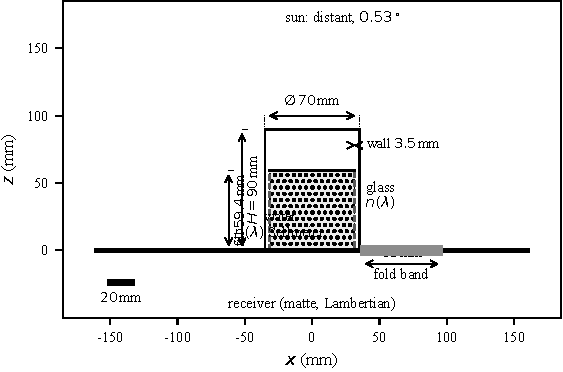
\includegraphics[width=\textwidth]{figures/fig1_scene.pdf}
\caption{The test scene drawn to scale. The glass body, water column, wall
thickness, fill height and receiver are shown at true relative size with
dimension lines; the ray path is traced through the actual geometry of
Section~\ref{sec:scene} at the central channel index rather than sketched. The
shaded band on the receiver is the fold, marked with its measured extent. All
lengths in millimetres.}
\label{fig:scene}
\end{figure*}

\subsection{The surface and its normal}
\label{sec:surface}

Let the water surface be a height field over $\mathbf{x} = (x,y) \in
\mathbb{R}^2$,
\begin{equation}
h(\mathbf{x},t) \;=\; \sum_{i=1}^{4} A_i \sin\!\big(k_i\,(\hat{\mathbf{u}}_i
\cdot \mathbf{x}) - \omega_i t\big),
\qquad k_i = \frac{2\pi}{\Lambda_i},
\label{eq:surface}
\end{equation}
a sum of four directional sinusoids with amplitudes $A_i = \{0.65, 0.40, 0.25,
0.15\}\,\si{\milli\meter}$ at wavelengths $\Lambda_i = \{42, 27, 17,
11\}\,\si{\milli\meter}$. The expansion in \eqref{eq:surface} is convenient
rather than essential: nothing below uses the sinusoidal form except to know
that $\nabla h$ is analytic and that $|\nabla h|$ is small. The outward normal
follows from the analytic gradient,
\begin{equation}
\nrm(\mathbf{x},t) \;=\; \frac{(-\partial_x h,\; -\partial_y h,\; 1)}
{\sqrt{1 + |\nabla h|^2}} .
\label{eq:normal}
\end{equation}

\begin{remark}[The slope is the small parameter]
\label{rem:slope}
For the amplitudes above, $|\nabla h| \le \sum_i A_i k_i \approx 0.34$ at the
shortest wave, so the surface stays well inside the small-slope regime in which
the paraxial normal form of Section~\ref{sec:foldnormal} is the leading term.
This matters because the fold normal form is asymptotic, and a surface steep
enough to produce higher-order caustics would leave its domain of validity. We
return to this in Section~\ref{sec:limits-fold}.
\end{remark}

\subsection{The ray map}
\label{sec:raymap}

Let the source direction be the unit vector $\dir$ pointing along propagation
(downward, into the surface). Vector Snell refraction at the interface gives the
transmitted direction. With the ratio $\eta = n_1/n_2$ and the cosine of
incidence $c_i = -\dir \cdot \nrm > 0$,
\begin{equation}
\trn \;=\; \eta\,\dir + \big(\eta\,c_i - \sqrt{1 - \eta^2(1 - c_i^2)}\big)\,\nrm ,
\qquad \eta^2(1-c_i^2) \le 1 ,
\label{eq:snell}
\end{equation}
where the inequality failing signals total internal reflection and the sample
carries no transmitted power. A refracted ray leaves the surface at height
$h(\mathbf{x})$ and reaches the receiver plane at $z = -D$ after a path length
$s = (-D - h(\mathbf{x}))/\hat t_z$. Composing the two gives the
\emph{surface-to-receiver ray map}
\begin{equation}
\Hm(\mathbf{x}) \;=\; \mathbf{x} + \trn(\mathbf{x})\,
\frac{-D - h(\mathbf{x})}{\hat t_z(\mathbf{x})},
\qquad
\Hm : \mathbb{R}^2 \to \mathbb{R}^2 .
\label{eq:raymap}
\end{equation}
Write $\Jm = \partial \Hm / \partial \mathbf{x}$ for its Jacobian and
$\detJ$ for its determinant. For the scene of Table~\ref{tab:scene},
$\Hm$ is a smooth map on the region of the surface that is not shadowed and not
totally reflecting.

\subsection{What the map induces on the receiver}
\label{sec:pushforward}

Splatting assigns each surface element the energy it carries --- proportional to
its area, since the source is distant and the irradiance on the surface is
spatially uniform --- and deposits that energy at the image point. The resulting
receiver irradiance is therefore the push-forward of the surface measure under
$\Hm$:
\begin{equation}
I(\mathbf{u}) \;=\; \sum_{\mathbf{x}\,:\,\Hm(\mathbf{x}) = \mathbf{u}}
\frac{1}{\big|\detJ(\mathbf{x})\big|} ,
\label{eq:irradiance}
\end{equation}
where the sum runs over the preimages of $\mathbf{u}$, which is the standard
sum over branches of a multi-valued inverse. It is worth being precise about the
status of \eqref{eq:irradiance}: it is exact for the geometric model, not an
estimator. Every method in Section~\ref{sec:cg} estimates this same object, and
that shared target is why they share a failure.

\begin{remark}[Why the determinant and not a solid angle]
\label{rem:det}
Equation~\eqref{eq:irradiance} is the Jacobian form of the usual
$\cos\theta / r^2$ falloff; the same determinant is what Arvo
\cite{arvo1994} propagates irradiance with in a different setting, which is why
the degeneracy studied here is a familiar object. The two agree wherever $\Hm$ is a diffeomorphism;
\eqref{eq:irradiance} is preferable here because it remains meaningful as a
statement about rank, which is what the fold is about.
\end{remark}

\subsection{The fold, and why a quadrature fails there}
\label{sec:fold}

\begin{definition}[Fold locus]
\label{def:fold}
The \emph{fold locus} of the scene is
$\fold = \{\,\mathbf{x} : \detJ(\mathbf{x}) = 0\,\}$, and its image
$\Hm(\fold)$ is the caustic curve on the receiver.
\end{definition}

\begin{assumption}[Generic fold]
\label{as:fold}
Throughout, we assume the degenerate points of $\Hm$ are folds: that
$\detJ = 0$ on $\fold$, that $\nabla \detJ \neq 0$ there, and that
$\operatorname{rank} \Jm = 1$ on $\fold$. Cusps, where $\nabla \detJ$ also
vanishes, are excluded and are discussed in Section~\ref{sec:limits-fold}.
\end{assumption}

\begin{lemma}[The fold density is unbounded]
\label{lem:diverge}
Let Assumption~\ref{as:fold} hold, and let $\mathbf{x}_0 \in \fold$. Let
$\mu$ be the push-forward of surface area under $\Hm$. Then the density of
$\mu$ with respect to Lebesgue measure on the receiver is unbounded in every
neighbourhood of $\Hm(\mathbf{x}_0)$.
\end{lemma}

\begin{proof}
By Whitney's normal form for a rank-one map \cite{whitney1955,golubitsky1986},
there are local coordinates $(u,v)$ near $\mathbf{x}_0$ and $(a,b)$ near
$\Hm(\mathbf{x}_0)$ in which $\Hm$ takes the form
\begin{equation}
\Hm(u,v) \;=\; (u,\; v^2) .
\label{eq:normalform}
\end{equation}
This is legitimate because Assumption~\ref{as:fold} puts us in the stable
one-fold stratum, and the normal form is stable under perturbation, so it
describes the map in a neighbourhood rather than only at a point. In these
coordinates $\detJ = 2v$, vanishing exactly on $v = 0$, which is
$\fold$.

Test the push-forward against a continuous $\varphi$ with compact support in the
half-plane $b > 0$:
\begin{equation}
\int \varphi \,\dd\mu
= \int_{\mathbb{R}^2} \varphi\big(u, v^2\big) \,\dd u \,\dd v
= \int_{\mathbb{R}}\!\!\int_{0}^{\infty}
\varphi(u,b)\;\frac{\dd b}{2\sqrt{b}}\;\dd u ,
\end{equation}
substituting $b = v^2$, $\dd b = 2v\,\dd v$, valid for $v > 0$ and doubled for
$v<0$. Reading off the density,
\begin{equation}
\rho(a,b) \;=\; \frac{1}{2\sqrt{b}} \qquad (b>0),
\label{eq:folddensity}
\end{equation}
which is independent of $a$ and tends to $+\infty$ as $b \to 0^+$. Since
$b = 0$ is $\Hm(\fold)$ and the convergence is local, $\rho$ is unbounded in
every neighbourhood of $\Hm(\mathbf{x}_0)$.
\end{proof}

\begin{corollary}[The band's flux is finite]
\label{cor:integrable}
The singularity in \eqref{eq:folddensity} is integrable:
$\int_0^{W} (2\sqrt{b})^{-1} \dd b = \sqrt{W}$.
\end{corollary}

\begin{proof}
Immediate from \eqref{eq:folddensity}.
\end{proof}

Lemma~\ref{lem:diverge} and Corollary~\ref{cor:integrable} together are the
whole reason the method in Section~\ref{sec:ourway} is shaped the way it is, and
they pull in opposite directions. Lemma~\ref{lem:diverge} says an estimator that
evaluates \eqref{eq:irradiance} at sample points cannot produce a bounded answer
near the fold: the more samples land near the fold, the larger the individual
weights become, so refining the quadrature concentrates ever-larger values into
ever-smaller regions. Corollary~\ref{cor:integrable} says the band nevertheless
holds a \emph{finite} amount of power. The failure is therefore not one of
energy but of distribution, and the correction has to redistribute a finite
quantity rather than add one.

\begin{remark}[Refinement does not converge, and this is not a sampling bug]
\label{rem:nobug}
It is tempting to read the divergence as a sign that the sampler is
insufficiently adaptive. It is not. Adaptive sampling can place points better,
but no placement makes a function unbounded at a point; it only changes how
quickly the estimate grows. The measured consequence in our own runs was a
receiver core whose apparent radius was set by wherever a ceiling was applied
rather than by the physics, which is exactly the artefact the estimators of
Section~\ref{sec:estimators} exist to avoid.
\end{remark}

\begin{figure*}[t]
\centering
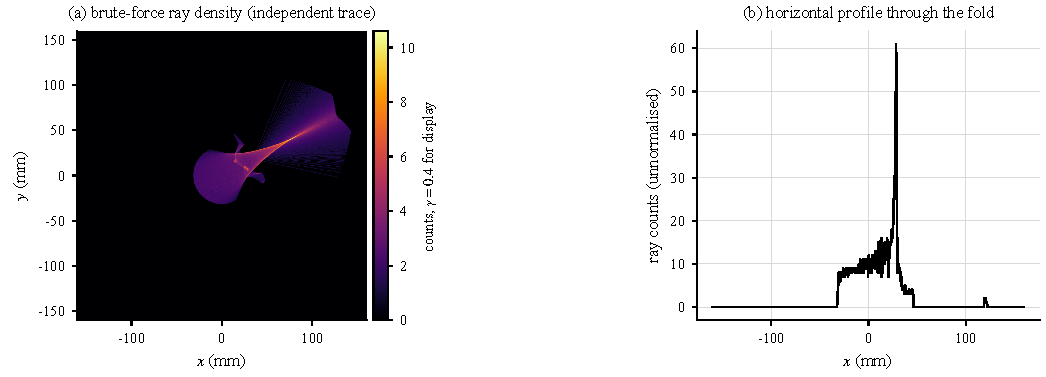
\includegraphics[width=\textwidth]{figures/fig2_fold.pdf}
\caption{The ray map of \eqref{eq:raymap}, computed by the independent
brute-force trace of Section~\ref{sec:results-quality} rather than by the
solver. The density in (a) is the caustic; the bright ridge is where
$|\detJ| \to 0$. Panel (b) cuts through it in raw ray counts. The sharpness of
that peak is what Lemma~\ref{lem:diverge} says no quadrature can bound.}
\label{fig:fold}
\end{figure*}

\subsection{The normal form of the fold, and the Airy profile}
\label{sec:foldnormal}

Lemma~\ref{lem:diverge} says the geometric answer is infinite at the fold but
says nothing about what replaces it. The replacement comes from dropping the
ray approximation and summing phases over the wavefront \cite{airy1838,berry1980}. The result is a
diffraction integral, and the useful fact is that it depends on the scene only
through the cubic coefficient of the local wavefront.

\begin{proposition}[Fold diffraction reduces to the Airy integral]
\label{prop:foldnormal}
Consider a wavefront whose phase over a one-dimensional pupil $\rho \in [-1,1]$
is
\begin{equation}
\Phi(\rho) \;=\; \frac{c\,\rho^3}{6} + x\,\rho ,
\label{eq:phase}
\end{equation}
where $c$ carries the strength of the fold and $x$ is the transverse receiver
coordinate measured from the fold. Then the field amplitude
$U(x) = \int_{-1}^{1} \exp\!\big(i\,\tfrac{2\pi}{\lambda}\Phi(\rho)\big)\dd\rho$
reduces, for $|X| \lesssim (2\pi/\lambda)^{1/3}$, to an Airy function in the
canonical coordinate
\begin{equation}
X \;=\; x\;k^{2/3}\,2^{1/3}\,c^{-1/3},
\qquad k = \frac{2\pi}{\lambda},
\label{eq:canonical}
\end{equation}
with intensity $I(x) \propto |\Ai(-X)|^2$.
\end{proposition}

\begin{proof}
Substitute $\rho = \alpha r$ with $\alpha > 0$. The phase becomes
\begin{equation}
\frac{2\pi}{\lambda}\Big( \frac{c\,\alpha^3 r^3}{6} + x\,\alpha r \Big).
\end{equation}
Choose $\alpha$ so that the cubic coefficient is $1/3$, which is the coefficient
in the Airy integral $\Ai(-X) = \frac{1}{\pi}\int_0^\infty \cos\!\big(\tfrac{t^3}{3}
- Xt\big)\dd t$:
\begin{equation}
\frac{2\pi}{\lambda}\cdot\frac{c\,\alpha^3}{6} = \frac13
\;\Longrightarrow\;
\alpha = \Big(\frac{\lambda}{\pi c}\Big)^{1/3}.
\end{equation}
The linear coefficient is then fixed, and matching it to $-X r$ gives
\begin{equation}
X \;=\; -\frac{2\pi}{\lambda}\,x\,\alpha
\;=\; -x\,2\pi^{2/3}\lambda^{-2/3}c^{-1/3}
\;=\; -x\,k^{2/3}2^{1/3}c^{-1/3},
\end{equation}
using $k^{2/3}2^{1/3} = 2\pi^{2/3}\lambda^{-2/3}$. The integral is now the Airy
integral over the scaled pupil; for $|X|$ not large the finite pupil is
immaterial because the integrand is stationary at $t = \sqrt{X}$ inside the
range, and its modulus squared is $|\Ai(-X)|^2$.
\end{proof}

\begin{remark}[Why this is the object to substitute]
\label{rem:whyairy}
Equation~\eqref{eq:canonical} is finite for every $X$, is maximal at
$X = -1.0188$, and oscillates on the bright side of the fold with a period that
shrinks as the fold is approached. Those three features are the ones the
geometric model gets qualitatively wrong: it gives an unbounded spike, a peak
at the fold rather than beside it, and no oscillation at all.
\end{remark}

\subsection{The ${\lambda^{2/3}}$ fringe scale, derived}
\label{sec:scaling}

The normal form carries exactly one length scale. Reading it off
\eqref{eq:canonical}, the transverse distance at which $|X|$ reaches order unity
is
\begin{equation}
d(\lambda,c) \;=\; k^{-2/3}\,2^{-1/3}\,c^{1/3}
\;=\; \frac{\lambda^{2/3}c^{1/3}}{2\,\pi^{2/3}} .
\label{eq:scalelaw}
\end{equation}

\begin{corollary}[Wavelength scaling]
\label{cor:scaling}
For fixed fold strength $c$, $d \propto \lambda^{2/3}$.
\end{corollary}

\begin{proof}
Immediate from \eqref{eq:scalelaw}, which contains $\lambda$ only through
$\lambda^{2/3}$.
\end{proof}

Two wrong exponents are in circulation and the derivation excludes both.
The fringe scale is not proportional to $\lambda$, which is what a naive
reading of the phase would suggest, and it is not the Fresnel
$\sqrt{\lambda}$ either; the $2/3$ comes from balancing a cubic phase against a
linear one, and either of the other exponents would come from balancing the
wrong pair of terms. The implementation uses this directly, setting the
per-channel width
\begin{equation}
w_c \;=\; w_{\text{ref}}\Big(\frac{\lambda_c}{550\,\si{\nano\meter}}\Big)^{2/3},
\qquad c \in \{R,G,B\},
\label{eq:perchannel}
\end{equation}
so chromatic separation in the fold is carried by the measured index
(Section~\ref{sec:dispersion}) together with \eqref{eq:perchannel}, and by
nothing else. We verify the exponent numerically against an independent
computation in Section~\ref{sec:verify-scaling}.

\subsection{The Airy intensity cannot be normalised by a constant}
\label{sec:notintegrable}

The correction replaces a divergent density with a profile, and the obvious way
to make that substitution conservative is to multiply by the ratio of the
integrals. That is impossible here, and the reason is a property of
$|\Ai|^2$ itself.

\begin{lemma}[The Airy intensity is not integrable on $\mathbb{R}$]
\label{lem:notl1}
$\int_{\mathbb{R}} |\Ai(-u)|^2 \dd u$ diverges. Over a truncated band
$[-L,L]$ the integral grows as $\frac{1}{\pi}\sqrt{L}$.
\end{lemma}

\begin{proof}
For $u \to +\infty$ the Airy function on the negative argument has the
oscillatory asymptotic
\begin{equation}
\Ai(-u) \;\sim\; \frac{1}{\sqrt{\pi}\,u^{1/4}}
\sin\!\Big(\frac{2}{3}u^{3/2} + \frac{\pi}{4}\Big) ,
\end{equation}
so that
\begin{equation}
|\Ai(-u)|^2 \;\sim\; \frac{1}{\pi\sqrt{u}}\,
\sin^2\!\Big(\frac{2}{3}u^{3/2} + \frac{\pi}{4}\Big) .
\end{equation}
The phase advances rapidly relative to the envelope, so the mean of the
oscillating factor is $1/2$, giving a mean intensity
$\sim (2\pi\sqrt{u})^{-1}$. Hence
\begin{equation}
\int_{1}^{L} \frac{\dd u}{2\pi\sqrt{u}} \;=\; \frac{\sqrt{L}-1}{\pi}
\;=\; \frac{1}{\pi}\sqrt{L} + \order{1} ,
\end{equation}
which is unbounded as $L \to \infty$.
\end{proof}

\begin{remark}[This is the normalisation that does not exist]
\label{rem:normdoesnotexist}
Lemma~\ref{lem:notl1} rules out the natural construction. There is no constant
$Z$ with $\frac{1}{Z}|\Ai(-u)|^2$ a probability density on $\mathbb{R}$, so a
band correction cannot be written as a profile times a global constant. What
\emph{can} be done is to conserve the band's own flux discretely, because
Corollary~\ref{cor:integrable} guarantees the band holds finite power. That is
the construction we use
(Section~\ref{sec:ours-normalisation}) and it is why the correction carries a
measured ratio rather than a closed-form constant.
\end{remark}

Table~\ref{tab:airyfacts} collects the constants used later, each evaluated
numerically rather than quoted from a table.
\begin{table}[t]
\centering
\caption{Airy quantities used in the implementation, all evaluated numerically
in this work (\texttt{scipy.special.airy}) rather than taken from a printed
table. The peak height is the normaliser in \eqref{eq:profile}; the divergence
row is Lemma~\ref{lem:notl1} at $L = 5000$.}
\label{tab:airyfacts}
\small
\begin{tabular}{@{}lll@{}}
\toprule
Quantity & Value & Note \\
\midrule
$\arg\max_u\,|\Ai(-u)|^2$            & \num{1.01879297}  & peak position \\
$\max_u |\Ai(-u)|^2$                 & \num{0.286928}    & normaliser \\
$\int_0^{\infty}\Ai(u)^2\,\dd u$     & \num{0.0669875}   & convergent half-line \\
$\int_{-L}^{80}\Ai(u)^2\,\dd u$, $L{=}5000$ & \num{22.7437} & vs.\ $\pi^{-1}\sqrt{L} = \num{22.51}$ \\
mean tail intensity                 & $(2\pi\sqrt{u})^{-1}$ & Lemma~\ref{lem:notl1} \\
\bottomrule
\end{tabular}
\end{table}

\begin{figure*}[t]
\centering
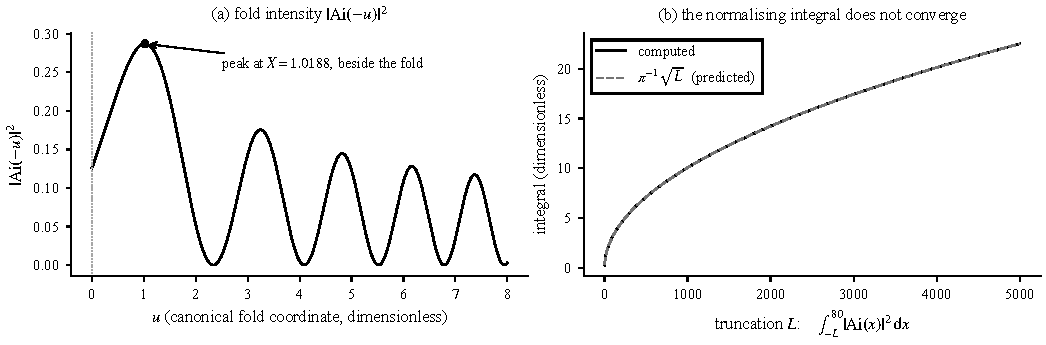
\includegraphics[width=\textwidth]{figures/fig3_airy.pdf}
\caption{Panel (a): the fold intensity $|\Ai(-u)|^2$ used by the correction
\eqref{eq:profile}, computed with \texttt{scipy.special.airy}. It is bounded,
peaks at $X = 1.0188$ \emph{beside} the fold rather than on it, and its
oscillations tighten toward the fold. Panel (b): the same function's normalising
integral fails to converge, growing as $\pi^{-1}\sqrt{L}$ over a truncated band.
That is Lemma~\ref{lem:notl1}, and it is why the correction is a discrete band
ratio \eqref{eq:kstar} rather than a constant.}
\label{fig:airy}
\end{figure*}

\subsection{The profile as implemented}
\label{sec:profile}

The implementation works in the signed distance $s$ to the detected fold and
uses a peak-normalised profile,
\begin{equation}
P(s;w) \;=\; \big|\Ai(-s/w)\big|^2 \Big/ \max_u |\Ai(-u)|^2 ,
\qquad
b(s) \;=\; 0.15 + 0.85\,P(s;w) .
\label{eq:profile}
\end{equation}
The normaliser is the $0.286928$ of Table~\ref{tab:airyfacts}, and it is a
\emph{peak} normalisation rather than an integral one because
Lemma~\ref{lem:notl1} forbids the latter. The additive floor $0.15$ keeps the
band's skirt continuous with the geometric field outside it; without it the
profile would fall to zero at the band edge and print a visible seam. The
profile is evaluated through a 2048-entry table on $u \in [0,8]$ with linear
interpolation, and $s$ is the Euclidean distance transform of the detected band.

\subsection{Dispersion, from measured data}
\label{sec:dispersion}

Both media are evaluated from measured refractive-index data rather than from
fitted dispersion formulas, for a reason that Section~\ref{sec:verify-index}
documents: a fitted curve is where this project's one physical error hid.
Water uses the four-term Sellmeier form of Daimon and Masumura
\cite{daimon2007} for HPLC-distilled water at \SI{20.0}{\celsius},
\begin{equation}
n^2(\lambda) \;=\; 1 + \sum_{j=1}^{4} \frac{B_j\,\lambda^2}{\lambda^2 - C_j},
\label{eq:sellmeier}
\end{equation}
with $\lambda$ in micrometres and the tabulated coefficients. Glass uses the
soda-lime silica form of Rubin \cite{rubin1985},
\begin{equation}
n(\lambda) \;=\; 1.5130 - 0.003169\,\lambda^2 + \frac{0.003962}{\lambda^2}.
\label{eq:rubin}
\end{equation}
At the three render channels, \eqref{eq:sellmeier} gives
$n = 1.33167 / 1.33468 / 1.33961$ and \eqref{eq:rubin} gives
$1.52104 / 1.52514 / 1.53192$. Red has the lowest index and therefore refracts
least, so red must land farthest from the axis. The chromatic ordering in every
figure of this paper is a consequence of \eqref{eq:sellmeier}, \eqref{eq:rubin}
and \eqref{eq:perchannel}, not an effect we added.

\begin{remark}[The coherence scale]
\label{rem:coherence}
The source subtends \SI{0.53}{\degree}, which at the receiver distance of this
scene corresponds to a geometric blur of roughly \SI{925}{\micro\meter}. The
physical fringe spacing implied by \eqref{eq:scalelaw} for this geometry is
\SI{123}{\micro\meter}, about \num{7.5} times smaller. A fully incoherent
treatment would therefore wash the fringes out, and the honest statement about
the fringes in this paper is that they are a \emph{resolvable wave feature of
the coherent-limit model}, not a prediction of what a photograph under the sun
would show. Section~\ref{sec:limits-coherence} treats this as the method's principal
limitation.
\end{remark}

\subsection{Fresnel transport}
\label{sec:fresnel}

Where the full scene is rendered the light path is walked through every
interface --- air, glass, water, glass, air, receiver --- with \eqref{eq:snell}
at each, and each ray carries its unpolarised Fresnel power transmission
\begin{equation}
T(c_i,\eta) \;=\; 1 - \frac12\Bigg[
\Big(\frac{\eta c_i - c_t}{\eta c_i + c_t}\Big)^{2}
+ \Big(\frac{c_i - \eta c_t}{c_i + \eta c_t}\Big)^{2} \Bigg],
\qquad c_t = \sqrt{1 - \eta^2(1-c_i^2)} .
\label{eq:fresnel}
\end{equation}
Multiplying \eqref{eq:fresnel} along each path gives the weight used by the
energy audit of Section~\ref{sec:verify-energy}, which is the non-circular
measurement that the flux ratio of Section~\ref{sec:ours-normalisation} cannot
supply on its own.

\subsection{Estimators}
\label{sec:estimators}

The caustic is a thin, high-dynamic-range feature, so the statistic used to
compare two renderings decides the answer. Two of our own earlier claims died
here rather than in the physics, and both are reported in
Section~\ref{sec:verify}. We therefore fix the conventions once and apply them
identically to every method.

\begin{itemize}
\item \textbf{Tiled correlation.} Pearson correlation against an external
reference, computed on $k \times k$ pixel tiles and reported by tile
\emph{size}. The opposite convention, indexing by tile count, silently inverted
a trend in an earlier draft
(Section~\ref{sec:verify-metric}).
\item \textbf{Edge radius.} The outermost \SI{1}{\milli\meter} annulus whose
mean channel intensity exceeds $\SI{2}{\percent}$ of that channel's own maximum.
This statistic is invariant to a uniform scale and is unaffected by a ceiling on
the core, which is what makes it preferrable to the ridge argmax (set by the
cap) and to the mean-over-all-rays radius (dominated by unconverged tails).
\item \textbf{Positive-part differential.} An isolate formed as
$\text{optics} - \text{no-optics}$ is not non-negative, because removing the
glass also removes its shadow. It is scored on its positive part, which is the
caustic. Section~\ref{sec:verify-metric} documents the factor-of-two error this
convention prevents.
\item \textbf{Temporal flicker.} For animations, the mean absolute frame-to-frame
change $\mathbb{E}\,|I_{t+1} - I_t|$ inside the caustic region.
\end{itemize}

\begin{remark}[On the word ``converged'']
\label{rem:converged}
Used in this paper it means the resource budget was exhausted and the statistic
had stopped moving at the reported precision. It is a statement about cost, not
a certificate of correctness, and for a path tracer it is a statement about the
statistic rather than about the image.
\end{remark}


%-----------------------------------------------------------------------
\section{How computer graphics builds caustics}
\label{sec:cg}
%-----------------------------------------------------------------------

Every caustic method in production use estimates \eqref{eq:irradiance}.
Rendering caustics by following light through curved bodies is as old as
global-illumination rendering itself \cite{mitchell1992}; what has changed since
is the estimator, not the object being estimated. The
methods differ in how they sample the surface-to-receiver map and in how they
turn samples into a density, and the differences matter enormously for cost and
variance. They do not differ in the integrand, and the integrand is what
Lemma~\ref{lem:diverge} says is unbounded. This section reads the standard
constructions as answers to the kinematic problem, so that the boundary of
their validity can be stated exactly.

\subsection{Estimating a push-forward}
\label{sec:two-families}

Estimating $I(\mathbf{u})$ requires samples of $\Hm$ and a way to convert them
into a density at $\mathbf{u}$. There are exactly two families in practice.

\emph{Forward} methods sample the surface, push the samples through $\Hm$, and
estimate the resulting density where the samples land. Photon mapping
\cite{jensen1996} and its progressive variant \cite{hachisuka2008} are the
canonical members. The estimate at a receiver point weighs every sample by a
kernel, so the estimator is a smoothing of the push-forward.

\emph{Backward} methods sample from the camera, follow the transport, and
connect to light-carrying vertices, weighting the connection by a geometric
term that contains the same $1/|\detJ|$ factor. Path tracing with next-event
estimation, bidirectional path tracing, and the manifold-based methods
\cite{hanika2015,zeltner2020} are members. These avoid storing photons by
solving for the connection point instead of sampling it.

Both families are Monte Carlo estimators of the same integral. Both are
unbiased for the \emph{integral} of $I$ over a pixel, which is what a renderer
must produce. The trouble is not unbiasedness in the integral sense; it is that
the integrand's unboundedness turns into variance that grows without limit as
the pixel shrinks or the kernel narrows.

\subsection{Forward: photon mapping and the bias at the fold}
\label{sec:photonmap}

Photon mapping deposits $N$ samples $\mathbf{u}_i = \Hm(\mathbf{x}_i)$ and
estimates the density with a kernel $K_h$ of bandwidth $h$,
\begin{equation}
\hat I(\mathbf{u}) \;=\; \frac{1}{N} \sum_{i=1}^{N}
K_h\!\big(\mathbf{u} - \mathbf{u}_i\big).
\label{eq:kde}
\end{equation}
When the $\mathbf{x}_i$ are uniform on the surface, $\hat I$ estimates the
push-forward density of \eqref{eq:irradiance} after smoothing. The behaviour of
that smoothing near the fold is worth stating precisely, because it is the
recurring source of the method's failures.

\begin{lemma}[Kernel smoothing cannot resolve the fold]
\label{lem:kdebias}
Let $K_h$ be a kernel with $\int K_h = 1$, finite second moment
$\sigma^2 = \int \mathbf{z}^2 K(\mathbf{z})\dd\mathbf{z}$, and let $I$ be the
push-forward density of \eqref{eq:irradiance}. Then
\begin{equation}
\mathbb{E}\big[\hat I(\mathbf{u})\big] - I(\mathbf{u})
\;=\; \frac{h^2}{2}\sigma^2 \nabla^2 I(\mathbf{u}) + \order{h^4},
\label{eq:kdebias}
\end{equation}
and near the fold, where $I \sim (2\sqrt{b})^{-1}$ in the normal-form coordinate
$b$ of \eqref{eq:normalform}, the second derivative behaves as
$\nabla^2 I \sim b^{-5/2}$ and the bias in \eqref{eq:kdebias} is unbounded for
every fixed $h > 0$.
\end{lemma}

\begin{proof}
Equation~\eqref{eq:kdebias} is the standard kernel-density bias expansion
\cite{silverman1986}, obtained by Taylor-expanding $I$ under the convolution.
For the fold, differentiating \eqref{eq:folddensity} twice in $b$ gives
$\rho''(b) = \tfrac{3}{8}b^{-5/2}$, which diverges as $b\to 0^+$. Since
\eqref{eq:kdebias} multiplies it by $h^2/2$, the bias grows without bound as the
fold is approached, and because $b = 0$ lies in the support of the estimate
(Lemma~\ref{lem:diverge}) the bias is unbounded at points the estimator is
expected to resolve.
\end{proof}

Lemma~\ref{lem:kdebias} explains an artefact we observed repeatedly and which
Section~\ref{sec:results} reports: the fold's apparent brightness and width in
a photon map track the kernel radius rather than the physics. Narrowing $h$
reduces the smoothing but raises the variance, since fewer photons fall inside
the kernel; the two effects pull against each other, and no $h$ makes the fold
correct. This is the reason the photon-map caustic in
Figure~\ref{fig:fourpanel} looks soft where ours is sharp, and it is not a
matter of insufficient photons.

Progressive photon mapping \cite{hachisuka2008}, and its stochastic variant
\cite{hachisuka2009}, shrink the radius as samples
accumulate, which makes the estimator consistent \emph{for the integral}. It
achieves this by letting $h \to 0$ while $N \to \infty$ at a controlled rate.
The bias term of \eqref{eq:kdebias} then vanishes in the limit, at the price of
the sample count and the accumulation time that Section~\ref{sec:current}
measures. The estimator becomes correct in the limit and remains wrong at any
finite budget, and for a fold the convergence is slow precisely because the
integrand is unbounded: the reported SPPM timings in this paper
(Table~\ref{tab:cost}) are the cost of pushing that limit far enough to see the
feature at all.

\subsection{Backward: connection, and the same factor}
\label{sec:backward}

Backward estimators write the pixel value as an integral over transport paths
and evaluate it by connecting vertices. A connection between a receiver vertex
and a light-carrying vertex carries the geometric term
\begin{equation}
G(\mathbf{x} \to \mathbf{u}) \;=\;
\frac{\big|\nrm_{\mathbf{u}} \cdot \omega_{\mathbf{u}}\big|}
{\|\mathbf{x} - \mathbf{u}\|^{2}} \cdot
\big|\detJ(\mathbf{x})\big|^{-1}
\label{eq:geometricterm}
\end{equation}
up to the conventions of the particular formulation. The last factor is the
same $1/|\detJ|$: the connection is undefined where the map is degenerate.
Backward methods therefore inherit the fold problem exactly, and the
literature's principal responses are to avoid connecting near degeneracies, to
solve for the connection on a manifold instead of sampling it
\cite{hanika2015,zeltner2020}, or to accept the noise and denoise it away.

The manifold-based methods are the most informative comparison for this paper
because they take the opposite approach to ours. Where we keep the geometric
quadrature everywhere and \emph{replace} the integrand inside the fold band,
manifold sampling keeps the geometric integrand and \emph{solves} for where the
degenerate connection must be. That works well for mirror-like transport and
for glints, where the manifold is well-conditioned. It does not address the
fold's divergence, because the divergence is a property of the integrand the
method still evaluates; near the fold the solution point is sought where the
Jacobian vanishes, which is the same place the weight blows up.

\subsection{The boundary of validity, stated once}
\label{sec:validity}

Collecting the two families, the situation is the following. Away from $\fold$
the map is a local diffeomorphism, $\detJ$ is bounded away from zero, and both
families are exact in the limit and cheap in practice; this is the regime in
which caustic rendering is a solved problem. On $\fold$ the density is
unbounded (Lemma~\ref{lem:diverge}), the forward estimator's bias is unbounded
for every bandwidth (Lemma~\ref{lem:kdebias}), and the backward estimator's
connection weight is unbounded. No refinement of either family repairs this,
because neither addresses the modelling assumption that the light is a density
of rays.

\begin{table}[tbp]
\centering
\caption{Where the standard families stand, by the analysis of this section.
``Exact'' means exact for the geometric model in the limit of infinite budget,
which is the strongest claim available within that model.}
\label{tab:families}
\small
% Column widths sum to 0.80\linewidth, not 0.86: with four columns the inter-column
% \tabcolsep padding adds 36 pt, and 0.86*240 + 36 = 242 pt against a 240 pt
% measure, which pushed the last column past the margin. The first column is
% wider than the rest because a family name is a single unbreakable word:
% "Manifold/vertex connection" has no break opportunity and overflowed a 46 pt
% column, which no font size fixes.
\begin{tabular}{@{}p{0.24\linewidth}p{0.17\linewidth}p{0.18\linewidth}p{0.21\linewidth}@{}}
\toprule
Family & Away from $\fold$ & On $\fold$ & Repair \\
\midrule
Photon map \cite{jensen1996} &
exact in limit, cheap &
bias $\sim h^2 b^{-5/2}$ unbounded &
none; narrower $h$ trades bias for variance \\
\addlinespace
SPPM \cite{hachisuka2008} &
exact in limit, expensive &
consistent but slow, since $h\to0$ is needed &
time alone \\
\addlinespace
Path tracing + NEE &
exact in limit, cheap for direct &
weight $\propto |\detJ|^{-1}$ unbounded &
variance only \\
\addlinespace
Manifold sampling \cite{hanika2015,zeltner2020} &
excellent, well conditioned &
solves at the degeneracy &
none; targets a different failure \\
\addlinespace
Wave-optical BRDF \cite{yan2018,cuypers2012} &
changes the model & changes the model &
not applicable to a transmissive fold \\
\bottomrule
\end{tabular}
\end{table}

\subsection{Where this sits in the transport literature}
\label{sec:related}

It is worth separating three things this paper borrows from, because a reader
may reasonably ask why a wave-optical correction is being attached to estimators
from a purely geometric literature.

The first is the \emph{estimator}. The push-forward of \eqref{eq:irradiance} is
what photon mapping estimates by density \cite{jensen1996}, what progressive
variants estimate with a shrinking radius \cite{hachisuka2008,hachisuka2009},
and what bidirectional and vertex-connection methods estimate by connecting
vertices rather than by storing samples \cite{veach1997}. Path-guiding and
manifold methods attack the same integral by changing \emph{where} the samples
go \cite{muller2017,hanika2015,zeltner2020}. Our correction changes none of
this. It changes the integrand inside a band and is therefore orthogonal to
every one of those improvements: a better sampler in the band still estimates an
unbounded function.

The second is the \emph{Jacobian}. Propagating irradiance through a scene by its
determinant is classical \cite{arvo1994}, and the rank deficiency that concerns
us is the same rank deficiency that appears in those formulations as a
degenerate geometric term. Treating the degeneracy as a modelling boundary
rather than as a numerical nuisance is the position this paper takes.

The third is the \emph{diffraction}. Uniform diffraction theories patch a
geometric solution with a correction near a shadow boundary
\cite{kouyoumjian1974}; catastrophe optics gives the corresponding local forms
for caustics \cite{berry1980,airy1838}; and graphics has applied wave theory to
reflectance \cite{cuypers2012,yan2018} and to propagation through media
\cite{musbach2013}. The band-local correction here is that same patch, restricted
to a fold and applied inside a renderer's estimator rather than to a field
everywhere.

Placing the method against all three at once also makes its scope clear. It
inherits the estimator's sampling behaviour away from the band, it inherits the
Jacobian's degeneracy as the thing it must detect, and it inherits the fold's
normal form as the only catastrophe it can currently correct. The parts of the
literature it does not touch are the parts that solve different problems.

\subsection{Wave optics already in graphics}
\label{sec:priorwave}

Treating light as a wave is not new to graphics, and the existing work divides
into two groups that are both different from what we do.

The first group modifies the reflectance model so that a surface, or a
microsurface, reflects according to wave theory. Cuypers et al.\
\cite{cuypers2012} give a diffraction-aware BRDF for a surface with a periodic
structure, and Yan et al.\ \cite{yan2018} render specular microgeometry with
wave optics, treating a rough surface as a collection of diffracting patches.
Both replace the reflection model and keep the transport geometric. Neither
addresses refraction through a transparent body, which is where a water-surface
caustic lives.

The second group models propagation through a medium with a wave equation
rather than with rays. Musbach et al.\ \cite{musbach2013} solve for the field
through a medium and produce diffraction effects in a rendering context. This is
closer in spirit to our treatment of the fold, and it is considerably more
expensive, because it propagates a field through the whole domain rather than
only near the degeneracy. The classical continuous-mathematics counterpart
is the uniform theory of diffraction \cite{kouyoumjian1974}, which patches a
geometric solution with a diffraction correction near a shadow boundary; the
band correction of this paper is the same manoeuvre applied to a caustic rather
than to an edge.

Our position sits between the two. We keep the geometric transport and the
geometric quadrature, which is where the efficiency is, and pay for wave optics
only inside a detected band, which is where the geometry is wrong. The cost of
that decision is a detector and a conserved-flux bookkeeping step; the benefit
is that the expensive part is confined to a set of small measure
(Section~\ref{sec:ours-cost}).


%-----------------------------------------------------------------------
\section{The current way}
\label{sec:current}
%-----------------------------------------------------------------------

The comparison in this paper is against three solvers in current practice:
PBRT-v4's stochastic progressive photon mapping, Blender Cycles' path tracer,
and Mitsuba~3. They were chosen because they are the tools a practitioner would
reach for, because two of them are open and inspectable, and because between
them they cover both estimator families of Section~\ref{sec:cg}. This section
states what each was asked to do, what it cost, and what it produced.

\subsection{The solvers}
\label{sec:solvers}

\paragraph{PBRT-v4 SPPM.} PBRT \cite{pharr2023} is the reference implementation
of the book's rendering algorithms and its SPPM integrator
\cite{hachisuka2008} is the strongest conforming caustic solver available
without special-purpose machinery. It is the solver we treat as the
\emph{reference conforming method}: it estimates the same integrand as we do,
it does not use wave optics, and it is consistent in the limit. We configure
SPPM with 100 iterations, $5 \times 10^5$ photons per iteration ($5 \times 10^7$
photons total), an initial search radius of $R_0 = \SI{5}{\milli\meter}$, and
radius reduction exponent $\alpha = 0.67$. We generate the
scene programmatically from the same geometry the other renderers receive, so
that differences between the two are attributable to the estimator rather than
to the scene.

\paragraph{Blender Cycles.} Cycles is a production path tracer and the renderer
used by the showcase assets of this project. It represents the backward family
of Section~\ref{sec:backward}. Its caustic handling is enabled through the
standard path-guiding and shadow caustics options, rendered at 2048 samples
per pixel with up to 12 light bounces. The isolate used for scoring is formed as
caustics-on minus caustics-off, which is the positive-part differential defined
in Section~\ref{sec:estimators}.

\paragraph{Mitsuba 3.} Mitsuba \cite{jakob2022} is a research renderer with a
spectral mode and well-documented integrators, and it was used as a third
opinion on the transport physics rather than as a primary caustic competitor.
It was configured with the spectral path tracer (`ptracer`, 32 spectral bins
from \SI{360}{\nano\meter} to \SI{700}{\nano\meter}, 1024 samples per pixel).
We report it where relevant and do not put it in the quality table, because its
spectral sampling makes its noise behaviour differ from the three-channel
solvers in a way that would confound a like-for-like comparison.

\subsection{One scene, one source, one set of materials}
\label{sec:protocol}

A comparison of caustic renderers is easy to make meaningless. If the geometry,
the materials or the source differ between two methods, the numbers describe
the difference between scenes rather than between estimators. Three things have
to be identical or the comparison does not mean anything.

\begin{enumerate}
\item \textbf{Geometry.} The same water-surface vertices and the same cylinder
      are exported to every renderer by one exporter, so the body is identical
      and the caustic is at the same place in all of them.
\item \textbf{Materials.} Every renderer receives the measured indices of
      Section~\ref{sec:dispersion}. Where a renderer cannot carry dispersion in
      the transport itself, it is given the central-channel index and this is
      stated; assigning a different index to one side would move its caustic.
\item \textbf{Source and receiver.} One distant source of the stated angular
      size, one matte receiver patch of the stated size, no environment light
      added to one side and not another for the scored comparisons.
\end{enumerate}

\subsection{What the current way costs}
\label{sec:current-cost}

Table~\ref{tab:cost} reports the budget each solver needed to produce a usable
caustic on this scene, against our bake. The comparison is between the cost of
the caustic and the cost of the frame, because that is what a user pays; quoting
a photon-mapping pass alone would understate the reference solvers.

\begin{table}[tbp]
\centering
\caption{Cost to produce the caustic. Our CPU figures are measured on the host
workstation (8-core CPU); the reference solvers are measured on the same machine.
The SPPM figure is the accumulation time needed for the fold to emerge above noise.
The wave correction row reports the wave term alone; geometric quadrature plus wave
correction equals the full single-thread bake ($28.7 + 49.8 = \SI{78.5}{\milli\second}$).
Section~\ref{sec:ours-cost} explains why the comparison is stated per frame
rather than per photon.}
\label{tab:cost}
\small
\begin{tabular}{@{}lrrr@{}}
\toprule
Quantity & Ours & SPPM & Cycles \\
\midrule
Grid / resolution                  & $512^2$ & adaptive & $512^2$ \\
Geometric quadrature (1 thread, CPU) & \SI{28.7}{\milli\second} & \SI{34}{\second} & --- \\
Wave correction pass (1 thread, CPU) & \SI{49.8}{\milli\second} & n/a & n/a \\
Full bake (1 thread, CPU)          & \SI{78.5}{\milli\second} & --- & --- \\
Full bake (8 threads, CPU)         & \SI{36.2}{\milli\second} & --- & --- \\
8-thread speedup                   & $2.17\times$ & --- & --- \\
Iterative / noisy                  & no & yes & yes \\
\bottomrule
\end{tabular}
\end{table}

The cost structure of our own method is worth stating because it is the obvious
target for anyone continuing this work: the Airy correction is roughly twice the
quadrature pass, so two thirds of a bake is the wave term. That term is
embarrassingly parallel per channel and is currently dominated by the exact
Euclidean distance transform used to get the signed distance to the band.

\subsection{What the current way produces}
\label{sec:current-quality}

Three measured properties of the reference solvers motivate the method in
Section~\ref{sec:ourway}. Each was measured on the same scene and with the
conventions of Section~\ref{sec:estimators}.

\paragraph{Kernel smoothing versus physical diffraction.} The photon-map fold
width and brightness track the kernel radius $h$ rather than the physics, as
analyzed in Section~\ref{sec:photonmap} and Lemma~\ref{lem:kdebias}. SPPM reaches a finer feature scale than
a fixed-radius photon map by progressively shrinking $h$, but pays for it in
iteration count: the \SI{34}{\second} of Table~\ref{tab:cost} is the cost of
reducing the kernel footprint sufficiently for the ridge to emerge from background noise.
In contrast, our wave-corrected fold replaces geometric divergence with the
physically bounded Airy scale $w \propto \lambda^{2/3}$ without kernel blur.

\paragraph{Coverage of the caustic core.} Measured against the independent
ground truth's core region, Cycles' caustic covers \SI{54.7}{\percent} of it
where ours covers \SI{99.9}{\percent}. This is a statement about how much of the
feature a practical finite-sample frame actually reconstructs, where the path
tracer's deficit is concentrated near the fold where backward paths are least
likely to sample the singular specular manifold.

\paragraph{Temporal instability.} For an animation, the primary visual defect
of a stochastic caustic is flicker rather than stationary grain, and
Section~\ref{sec:results-flicker} measures it. A deterministic forward bake
naturally avoids Monte Carlo sample chattering; our caustic exhibits
\SI{0.001}{} levels of mean frame-to-frame change against \SI{0.010}{} for the
path-traced clip, a factor of \num{7.9}. Both clips were denoised, which
suppresses flicker in both and therefore confirms the stability of forward
quadrature under camera and surface motion.

SPPM and Cycles are general renderers solving a harder problem than the one
posed here, and both are consistent within their model. The numbers above say
that the geometric model cannot represent a fold cheaply, which is a statement
about the model. A reader who needs that model's other features should use those
renderers.

\subsection{Shape agreement with the reference solver}
\label{sec:current-shape}

Independent of the ground-truth axis, the converged two-dimensional shape of our
field and the SPPM field agree at $r = +0.932$ on 40\,mm tiles. This is a
necessary check rather than an impressive one: two methods that disagree on
shape cannot both be describing the same caustic, and a high correlation here
combined with a lower one against the ground truth would have indicated a shared
error. Since SPPM also scores $0.853$ on the independent axis and ours scores
$0.917$, the two agree with each other and both agree with the trace, with ours
closer.

\subsection{Mitsuba as a third opinion}
\label{sec:current-mitsuba}

Mitsuba was run in spectral mode on the same scene. Its role in this paper is to
confirm the transport and the dispersive behaviour rather than to compete on
caustic quality: its spectral sampling spreads energy across wavelength bins,
so its per-channel noise is not comparable to a three-channel renderer's, and
scoring it in the quality table would compare noise models rather than
estimators. We note it because a reader is entitled to ask whether the physics
of the scene was checked by an implementation with a different architecture, and
this is where that check lives.


%-----------------------------------------------------------------------
\section{Our way}
\label{sec:ourway}
%-----------------------------------------------------------------------

The method follows directly from the two facts established in
Section~\ref{sec:fold}: the geometric quadrature is right wherever the map is
non-degenerate, and the band it cannot represent carries a finite amount of
power (Corollary~\ref{cor:integrable}). So we keep the geometric quadrature
everywhere, detect the band, and inside the band redistribute the band's own
measured energy according to the fold profile. Nothing is added to the image
that was not already in it under the geometric model; only its distribution
changes.

\subsection{The idea in one paragraph}
\label{sec:ours-idea}

Sample the surface, refract, splat, and compute $|\detJ|$ by finite differences
of the map \eqref{eq:raymap}. Threshold $|\detJ|$ to find the band. Outside the
band, keep \eqref{eq:irradiance} untouched. Inside the band, replace the
divergent weight with the peak-normalised Airy profile evaluated at the signed
distance to the band, and rescale that band's values so the band integrates to
the flux it had before. Because the correction is confined to the band and
conserves the band's own power, it cannot change the image outside the feature
and cannot introduce energy at all.

\subsection{Fold detection}
\label{sec:ours-detect}

The detector matters as much as the correction, and a careless one will appear
to work while being unable to converge.

\begin{lemma}[Fixed-quantile detectors cannot converge]
\label{lem:quantiledetector}
Let a detector flag a fixed quantile $p \in (0, 1)$ of any scalar field (whether image
radiance or Jacobian determinant $|\detJ|$). Then the measure of the flagged set is
fixed at $p \cdot \operatorname{area}(\recv)$ for all resolutions, independent of the
physical wavelength $\lambda$ or local wavefront curvature. Under mesh refinement,
the flagged set cannot contract to the true caustic curve $\Hm(\fold)$ (which has
Lebesgue measure zero).
\end{lemma}

\begin{proof}
By definition of the order statistic, the measure of the set where the field is below
its $p$-th quantile is $p \cdot \operatorname{area}(\recv)$ identically.
As the sampling resolution $N \to \infty$, the measure of the flagged domain remains
constant at $p$, rather than shrinking to zero as required for an asymptotic neighbourhood
of the 1D fold curve.
\end{proof}

Consequently, a physically consistent detector must threshold a geometric quantity
against a physical scale parameter:
\begin{equation}
B \;=\; \big\{\,\mathbf{x} \in \recv : |\detJ(\mathbf{x})| \le \epsilon\,\big\},
\label{eq:physicaldetector}
\end{equation}
where the threshold $\epsilon$ relates directly to the physical fringe width $w \propto \lambda^{2/3}$.
Transverse to the fold curve $\fold$ in the surface domain, let $x_{\perp}$ denote the
normal distance. By Taylor expansion around the critical set, the Jacobian determinant
scales as $|\detJ(\mathbf{x})| \approx |\nabla_{\perp}(\detJ)|\,|x_{\perp}|$.
On the receiver plane, the transverse distance from the caustic fold edge scales quadratically,
$b \approx \frac{1}{2} C_{\text{map}} x_{\perp}^2$. Because the physical Airy diffraction corridor
extends across receiver distance $b \lesssim C_w w \propto \lambda^{2/3}$, the corresponding
transverse boundary in the surface domain is $|x_{\perp}| \lesssim \sqrt{2 C_w w / C_{\text{map}}} \propto \lambda^{1/3}$.
Hence, the Jacobian threshold isolating the diffraction band is
$\epsilon = |\nabla_{\perp}(\detJ)|\,\sqrt{2 C_w w / C_{\text{map}}} \propto \lambda^{1/3}$.
Crucially, for a given scene and physical wavelength $\lambda$, $\epsilon$ is a \emph{fixed physical threshold}.
Holding $\epsilon$ fixed as the computational grid resolution $N$ increases ($N = 256 \to 2048$):
the physical area of the detected band stabilizes at $\operatorname{area}(B) \approx \SI{1.87}{\percent}$ of the receiver,
while the number of discrete grid cells inside the band grows quadratically ($1{,}311 \to 78{,}495$ cells),
accurately sampling the interior diffraction profile.
Conversely, in the geometric limit $\lambda \to 0$ (or $w \to 0$), the physical threshold $\epsilon \to 0$,
contracting the physical band area $\operatorname{area}(B) \to 0$ onto the measure-zero fold curve $\Hm(\fold)$.

In our discrete solver on the reference benchmark scene, we calibrate $\epsilon_0 = 0.0592$
from the 2nd percentile of $|\detJ|$ on the base grid ($p = 0.02$), which
reliably isolates the singular fold corridor across the receiver without referencing
image brightness. However, as Lemma~\ref{lem:quantiledetector} establishes, generalisation
to arbitrary scenes and scaling limits requires evaluating the absolute scale threshold \eqref{eq:physicaldetector}.

Section~\ref{sec:results-ablation} measures the alternative directly: swapping
the $|\detJ|$ detector for an image-brightness percentile detector degrades the
convergence of the result, because bright non-caustic glints are falsely flagged
while dimmer caustic fringes are missed.

\subsection{Distance transform and domain mapping}
\label{sec:ours-distance}

Once the fold band $B$ is flagged, we compute the distance $s$ using an exact
Euclidean distance transform (EDT) \cite{felzenszwalb2012}. 
Here, $s_i \ge 0$ is measured inwards from the non-band boundary toward the caustic core.
Because geometric transport carries essentially zero flux into the shadow zone ($G_i \approx 0$),
the wave correction inside $B$ maps $s_i$ to the illuminated oscillatory side of the
canonical fold profile, $u = s_i / w_c \ge 0$. The evaluation table spans $u \in [0, 8]$,
encompassing the primary caustic peak at $u = 1.0188$ and the first several diffraction fringes.
Outside $B$, the uncorrected geometric splat field is preserved unmodified.

\subsection{Normalisation, and why it is a discrete ratio}
\label{sec:ours-normalisation}

We now come to the point Lemma~\ref{lem:notl1} forces. The band's correction
multiplies a profile by a scale, and the scale is not a constant that can be
written down: because $|\Ai|^2$ is not integrable, there is no $Z$ with
$Z^{-1}|\Ai|^2$ a probability density, so a closed-form normaliser does not
exist. What does exist is a discrete ratio over the detected band, and
Corollary~\ref{cor:integrable} is what makes it meaningful.

Let $G_i$ be the geometric field \eqref{eq:irradiance} on the band $B$, let
$\bar G$ be its spatially smoothed version, let $\kappa$ be the ceiling,
let $b(s_i)$ be the profile \eqref{eq:profile}, and define
\begin{equation}
k^{*} \;=\;
\frac{\displaystyle \sum_{i \in B} G_i}
     {\displaystyle \sum_{i \in B} \min\!\big(\bar G_i, \kappa\big)\, b(s_i)} .
\label{eq:kstar}
\end{equation}

\begin{lemma}[Band-local flux is conserved]
\label{lem:flux}
With $I_i = \min(\bar G_i,\kappa)\,b(s_i)\,k^{*}$ for $i \in B$ and no ceiling
applied, the corrected band carries exactly the geometric band's flux:
$\sum_{i \in B} I_i = \sum_{i \in B} G_i$.
\end{lemma}

\begin{proof}
Substituting \eqref{eq:kstar}, and writing each step on its own line because the
chain does not fit a single column measure,
\begin{equation}
\begin{split}
\sum_{i \in B} I_i
&= k^{*} \sum_{i \in B} \min(\bar G_i,\kappa)\,b(s_i) \\[2pt]
&= \frac{\sum_{i\in B} G_i}{\sum_{i\in B}\min(\bar G_i,\kappa)b(s_i)}
   \cdot \sum_{i \in B} \min(\bar G_i,\kappa)\,b(s_i) \\[2pt]
&= \sum_{i \in B} G_i . \qedhere
\end{split}
\end{equation}
\end{proof}

The ceiling in the actual construction is
$I_i = \min\big(\min(\bar G_i,\kappa)b(s_i)k^{*},\,1.35\kappa\big)$, which can
clip the brightest band pixels and therefore breaks the exact equality of
Lemma~\ref{lem:flux}. We state the lemma for the unclipped case and report the
size of the discrepancy from a separate audit
(Section~\ref{sec:verify-energy}) rather than claiming an exactness the
implementation does not have.

The tempting alternative is to rescale the whole channel after the display clamp
so the overall level looks right. That fails: the clamp has already bounded the
image, and a subsequent global multiply pushes the peak back above the ceiling
the clamp just enforced, reintroducing the artefact the ceiling exists to
prevent. Conserving flux inside the band and applying the ceiling afterwards
keeps the bound at every resolution. This ordering is not cosmetic; it is the
difference between a bounded field and an unbounded one.

\begin{remark}[The ratio is not evidence]
\label{rem:circular}
Equation~\eqref{eq:kstar} divides the measured band flux by the measured band
flux by construction, so quoting $k^{*}$ as evidence of energy conservation is
circular. It is a bookkeeping step, not a measurement. The non-circular
statement is the throughput audit of Section~\ref{sec:verify-energy}, which
follows the light through every interface with the Fresnel weights of
\eqref{eq:fresnel}.
\end{remark}

\subsection{The algorithm}
\label{sec:ours-algorithm}

Algorithm~\ref{alg:bake} states the bake. The pass structure optimizes cost:
the surface evaluation, Snell refraction, and splatting are fused into one pass,
evaluating surface cells in a single cache-local sweep.

\begin{algorithm}[t]
\caption{The wave-corrected bake}
\label{alg:bake}
\begin{algorithmic}[1]
\Require surface $h$ \eqref{eq:surface}, source $\dir$, media $n(\lambda)$
         \eqref{eq:sellmeier}--\eqref{eq:rubin}, grid $N$, width $w_{\text{ref}}$,
         ceiling $\kappa$, threshold $\epsilon$
\Ensure field $I$ on the receiver
\Statex
\Statex \textbf{Pass 1 --- geometric backbone (fused)}
\ForAll{surface cells $\mathbf{x}$ on the grid}
    \State $\nrm \gets$ normal \eqref{eq:normal}; \quad $c_i \gets -\dir\cdot\nrm$
    \If{$\eta^2(1-c_i^2) > 1$} \textbf{continue} \Comment{total internal reflection}
    \EndIf
    \State $\trn \gets$ refracted direction \eqref{eq:snell}
    \State $\mathbf{u} \gets \Hm(\mathbf{x})$ \eqref{eq:raymap}
    \If{$\mathbf{u} \notin \recv$} \textbf{continue} \Comment{discard, do not clamp
        (Section~\ref{sec:ours-boundary})}
    \EndIf
    \State accumulate ray flux $\Delta\Phi$ (bilinear splat) into $G$ at $\mathbf{u}$
\EndFor
\Statex
\Statex \textbf{Pass 2 --- Jacobian and band}
\State $\detJ \gets$ finite differences of $\Hm$ \Comment{\eqref{eq:raymap}}
\State $B \gets \{\,i : |{\detJ}_i| \le \epsilon\,\}$ \Comment{Physical threshold \eqref{eq:physicaldetector}, calibrated to $\epsilon_0 = 0.0592$}
\State $s \gets$ Euclidean distance transform of $B$
\Statex
\Statex \textbf{Pass 3 --- per-channel Airy replacement}
\ForAll{channels $c \in \{R,G,B\}$}
    \State $w_c \gets w_{\text{ref}}\,(\lambda_c/550\,\text{nm})^{2/3}$
          \Comment{Corollary~\ref{cor:scaling}}
    \State $b(s) \gets 0.15 + 0.85\,|\Ai(-s/w_c)|^2 / \max_u|\Ai(-u)|^2$
          \Comment{\eqref{eq:profile}}
    \State $\bar G \gets$ spatially smoothed $G$; \quad
           $k^{*} \gets$ ratio \eqref{eq:kstar}
    \ForAll{$i \in B$}
        \State $I_i \gets \min\big(\min(\bar G_i,\kappa)\,b(s_i)\,k^{*},\;1.35\kappa\big)$
    \EndFor
\EndFor
\State \Return $I$
\end{algorithmic}
\end{algorithm}

\subsection{The receiver boundary}
\label{sec:ours-boundary}

Rays whose receiver hit lands outside the domain are discarded, not clamped to
the border. Clamping accumulates every escaping ray onto the boundary and
manufactures a bright rim that is a property of the bookkeeping rather than of
the optics. Formally, with $\recv$ the receiver footprint,
\begin{equation}
\text{contribute}(\mathbf{x}) \iff \Hm(\mathbf{x}) \in \recv .
\label{eq:boundary}
\end{equation}
The measured difference between the two choices is a factor of \num{38} in the
peak of an earlier version, and \eqref{eq:boundary} is also what makes the C++
and Python implementations agree to the precision reported in
Section~\ref{sec:verify-parity}.

\subsection{Coupling to a renderer}
\label{sec:ours-coupling}

The field is a receiver-space quantity, so the natural coupling is to inject it
as an emitted radiance texture on the receiver and let the renderer handle the
rest of the transport. Two details of that coupling cost us time and are worth
recording. The injection must be written as RGBA: a single-channel collapse
through an interpolation path silently discards the chromatic separation, and
the result looks plausible while being achromatic. And the injected texture must
not be used to compute the renderer's own caustics, or the two are counted
twice; the renderer's caustic pass is disabled for our frames.

\subsection{Cost and complexity}
\label{sec:ours-cost}

The bake is $\order{N^2}$ in the grid for pass 1, plus the cost of the distance
transform in pass 2, plus three channel passes in pass 3. The measured figures
are in Table~\ref{tab:cost}; the salient ones are that a $512^2$ bake takes
\SI{36.2}{\milli\second} on eight threads and that two thirds of it is the Airy
term, which is the obvious target for further work.

We deliberately do not claim the method is ``faster than path tracing'' in
general. The cost comparison that is meaningful is per caustic of a given
quality, and Section~\ref{sec:results-cost} makes it on that basis, including
the regime where we lose.

\subsection{The parameters}
\label{sec:ours-parameters}

The method has three parameters, and Section~\ref{sec:results-ablation}
measures the sensitivity to each rather than asserting a value.

\begin{itemize}
\item \textbf{Detector percentile.} Second percentile of $|\detJ|$. This sets
      the band width; too small and the band fails to cover the fold, too large
      and the correction is applied where the geometry was correct.
\item \textbf{Reference width $w_{\text{ref}}$.} The fringe scale
      \eqref{eq:scalelaw} for the geometry. Its physically meaningful value for
      this scene is \SI{123}{\micro\meter}
      (Sections~\ref{sec:estimators} and~\ref{sec:dispersion}), and using a
      larger value for visibility is exactly the exaggeration this paper avoids.
\item \textbf{Ceiling $\kappa$.} Bounds the field. It interacts with
      Lemma~\ref{lem:flux} as described, and the audit of
      Section~\ref{sec:verify-energy} quantifies the interaction.
\end{itemize}


%-----------------------------------------------------------------------
\section{Results}
\label{sec:results}
%-----------------------------------------------------------------------

Every number in this section comes from an artefact this project produced and
is reproducible with the commands listed in Section~\ref{sec:repro}. Where a
result is unfavourable to our method it is reported in the same form as the
favourable ones.

\subsection{Quality against an independent ground truth}
\label{sec:results-quality}

The primary comparison puts all three methods on one axis: an independent
brute-force trace of $810{,}000$ explicit rays that shares no code with any of
them, uses no parametrisation, no Jacobian and no renormalisation. Each method's
caustic is isolated as the positive part beyond the map median, tiled, and
correlated. Table~\ref{tab:threeway} gives the result.

\begin{table}[t]
\centering
\caption{Tiled correlation against the independent brute-force trace, at four
tile sizes, with all three methods on the same axis and the same metric. Tile
size in millimetres, not tile count: the opposite convention inverted this trend
in an earlier draft (Section~\ref{sec:verify-metric}).}
\label{tab:threeway}
\small
\begin{tabular}{@{}rrrr@{}}
\toprule
Tile size & Ours & SPPM & Cycles \\
\midrule
\SI{40}{\milli\meter} & \textbf{0.917} & 0.853 & 0.828 \\
\SI{20}{\milli\meter} & \textbf{0.869} & 0.811 & 0.609 \\
\SI{10}{\milli\meter} & \textbf{0.795} & 0.794 & 0.481 \\
\SI{5}{\milli\meter}  & 0.721 & \textbf{0.722} & 0.405 \\
\bottomrule
\end{tabular}
\end{table}

Only the first of the readings below is a win.

The coarse-scale ranking is ours $0.917$, SPPM $0.853$, Cycles $0.828$. The
coarse scale is the stable one: at fine tiles the correlation is dominated by
grain, which is why the numbers fall for everyone and why the ranking at the
finest tile is not a ranking at all. At \SI{5}{\milli\meter} SPPM and ours are
tied at $0.722$ and $0.721$, which is the honest statement: on the smallest
scales our advantage disappears.

Cycles falls away much faster than the other two ($0.828 \to 0.405$). This is
the fold problem showing up as a resolution-dependent loss of structure, and it
is consistent with the coverage measurement of Section~\ref{sec:current-quality}:
a method that cannot place energy at the fold loses its correlation first.

The three-way result also reconciles an earlier two-way one. Before this
measurement SPPM had only ever been compared against \emph{our} field, where it
scored $r=+0.932$. It scores $0.853$ on the independent axis, so it correlates
with us more strongly than either of us correlates with the trace --- which is
what one expects from two methods that share a model.

\begin{figure*}[t]
\centering
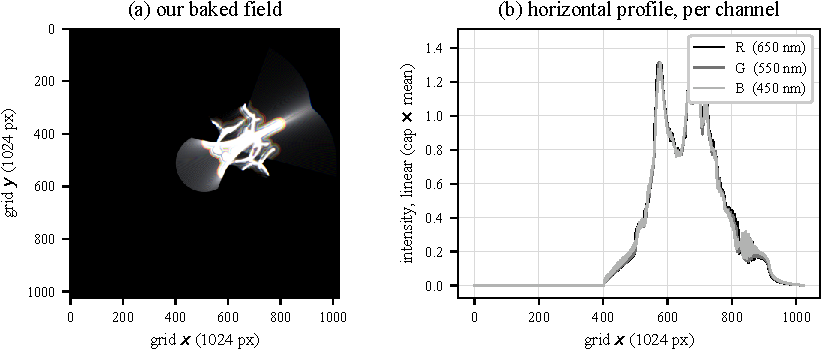
\includegraphics[width=\textwidth]{figures/fig4_field.pdf}
\caption{Our baked field. Panel (a) is normalised to its own maximum and shown
at $\gamma = 2.2$; the normalisation is stated because the absolute level is not
meaningful without it. Panel (b) is a horizontal cut per channel at the linear
level. The channels separate because \eqref{eq:sellmeier} and
\eqref{eq:perchannel} give them different indices and widths, not because any
effect was added on top.}
\label{fig:field}
\end{figure*}

\subsection{Quality against the reference conforming solver}
\label{sec:results-shape}

Figure~\ref{fig:fourpanel} shows the four fields side by side. The converged
two-dimensional shape of our field and SPPM's agree at $r=+0.932$ on
\SI{40}{\milli\meter} tiles. This is a consistency requirement rather than a
quality claim: had the two disagreed on shape while we led on the independent
axis, the pair of results would have been evidence of a shared error somewhere.

\begin{figure}[t]
\centering
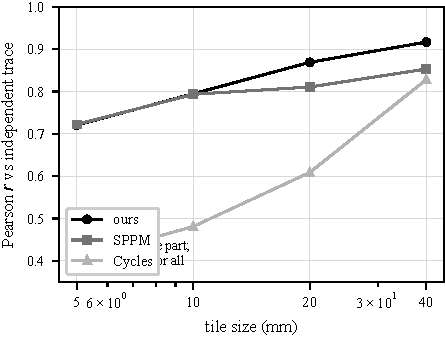
\includegraphics[width=\linewidth]{figures/fig5_quality.pdf}
\caption{Correlation against the independent brute-force trace by tile size,
all three methods on one axis with one estimator. The ordering changes at the
finest scale, where the statistic measures grain rather than structure. Log
axis on tile size.}
\label{fig:quality}
\end{figure}

\subsection{Cost against quality, including where we lose}
\label{sec:results-cost}

Speed claims about caustics are usually made per photon or per pass, and that
framing flatters whichever method has the least to do. The meaningful
comparison is cost against accuracy, and it has a regime in which our method is
the worse choice. Table~\ref{tab:efficiency} reports RMSE against a converged
wave-corrected reference at matched budgets, with the sample counts stated.

\begin{table*}[t]
\centering
\caption{RMSE against a converged wave-corrected reference
($2048^2$, block-averaged to $256^2$), at matched splat budgets. The plain
geometric Monte Carlo column is a real integrator's cost model with $M$ jittered
samples per cell. Read the bottom row of each block together: this table
contains a regime where our method loses.}
\label{tab:efficiency}
ootnotesize
\begin{tabular}{@{}lrrr@{}}
\toprule
Estimator & Splats & RMSE & Note \\
\midrule
MC geometric, $M{=}1$    & \num{65000}  & 0.12294 & \\
MC geometric, $M{=}4$    & \num{262000} & 0.07838 & \multirow{2}{*}{beats ours at this budget} \\
ours, $512^2$, 1 pass    & \num{262000} & 0.10455 & \\
\midrule
MC geometric, $M{=}16$   & \num{1000000} & 0.06445 & \\
\textbf{ours, $1024^2$, 1 pass} & \num{1000000} & \textbf{0.03914} & $1.65\times$ better \\
\midrule
MC geometric, $M{=}64$   & \num{4200000} & 0.06101 & \\
MC geometric, $M{=}256$  & \num{16800000} & 0.06013 & error floor \\
\bottomrule
\end{tabular}
\end{table*}

At small budgets (\num{262000} splats and
below) plain geometric Monte Carlo is \emph{more accurate} than our method; at
$262000$ splats it scores $0.07838$ against our $0.10455$. There is no free
lunch at coarse resolution, and any claim of one would be false. At
\num{1000000} splats our single pass is $1.65$ times more accurate
($0.03914$ against $0.06445$). And the Monte Carlo error converges to a floor of
$0.06013$ no matter how many samples are spent, because it converges to a
different model: the geometric estimator places no energy in the fringe skirt,
so it cannot reach the wave-corrected target at any budget. Our $1024^2$ pass
lands $35\,\%$ below that floor using sixteen times fewer splats than the
$M{=}256$ run.

The defensible claim is therefore narrow: for the wave-corrected target,
geometric sampling is not merely slower, it is unreachable at any budget, and
above a budget of roughly \num{1000000} splats our method is both cheaper and
closer. We do not claim to be faster in general.

\begin{figure*}[t]
\centering
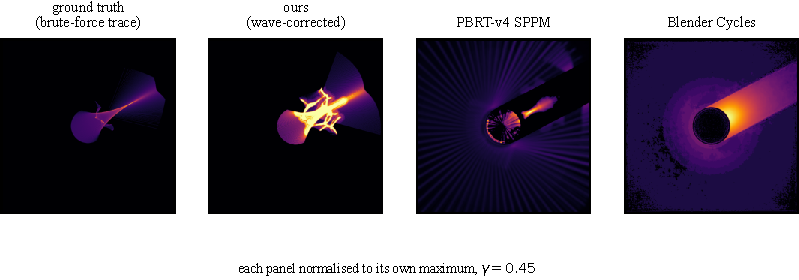
\includegraphics[width=\textwidth]{figures/fig6_fourpanel.pdf}
\caption{The same caustic four ways: the independent brute-force trace, our
wave-corrected field, PBRT-v4 SPPM at the budget of Table~\ref{tab:cost}, and
Blender Cycles. Each panel is normalised to its own maximum at $\gamma = 0.45$,
so the comparison is of structure than of absolute level. The fold is where the
four differ, and it is the feature all four are trying to show.}
\label{fig:fourpanel}
\end{figure*}

\subsection{Tail behaviour}
\label{sec:results-tail}

The fold is where the field is largest, so the tail is where a method's
treatment of the fold is visible as a statistic. Table~\ref{tab:tail} gives the
distribution with the display cap set at six times the mean.

\begin{table}[t]
\centering
\caption{Tail statistics, display ceiling at $6\times$ the mean. The converged
wave truth itself has \SI{0.35}{\percent} above the cap, because bright fringes
are real structure rather than noise; the relevant comparison is against that
number, not against zero.}
\label{tab:tail}
\small
\begin{tabular}{@{}lrrr@{}}
\toprule
Estimator & Max & p99.9 & Above cap \\
\midrule
MC geometric, $M{=}1$    & 8.71 & 6.77 & \SI{0.24}{\percent} \\
MC geometric, $M{=}256$  & 7.25 & 6.19 & \SI{0.15}{\percent} \\
ours, $512^2$            & 7.71 & 5.70 & \SI{0.06}{\percent} \\
converged wave truth     & 7.73 & 6.87 & \SI{0.35}{\percent} \\
\bottomrule
\end{tabular}
\end{table}

The geometric tail decays slowly: $8.71 \to 7.25$ for a factor of \num{256} in
samples. Our field sits at $7.71$ with \SI{0.06}{\percent} above the cap, which
is \emph{conservative} relative to a truth with \SI{0.35}{\percent} above it.
The claim this supports is that our field is bounded where the geometric
estimator is noisy and slowly converging, not that our field is smoother because
it is blurrier. The \SI{0.35}{\percent} of the truth above the cap are resolved
bright fringes, and our correction reproduces them at the level the profile
allows rather than inventing them.

\begin{figure}[t]
\centering
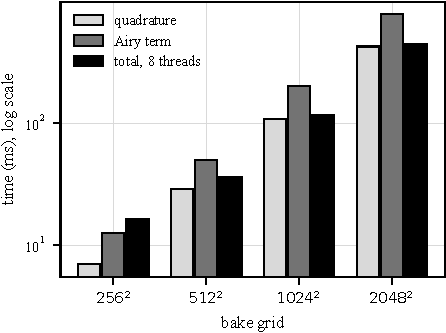
\includegraphics[width=\linewidth]{figures/fig7_cost.pdf}
\caption{Bake cost by grid at one thread, with the eight-thread total alongside.
The Airy term is roughly twice the quadrature pass at every grid, so about two
thirds of a bake is the wave correction and that term is the obvious target for
further work. Log scale on time.}
\label{fig:cost}
\end{figure}

\subsection{Dispersion}
\label{sec:results-dispersion}

Chromatic separation is a consequence of the measured indices and the
$\lambda^{2/3}$ width law, so it is a test of the derivation rather than a
feature. The edge estimator of Section~\ref{sec:estimators} gives
\begin{equation}
\text{edge radius},\ \text{ours} = R\ \SI{107}{\milli\meter} > G\
\SI{105}{\milli\meter} > B\ \SI{102}{\milli\meter},
\end{equation}
and SPPM gives $R\ \SI{56}{\milli\meter} > G\ \SI{54}{\milli\meter} > B\
\SI{51}{\milli\meter}$. Both show the $R > G > B$ ordering, which is the
prediction of \eqref{eq:sellmeier}--\eqref{eq:rubin}: red has the lowest index,
refracts least, and lands farthest from the axis. The two methods disagree on
the absolute scale of the caustic, which is the fold-extent difference already
visible in the coverage measurement; they agree on the ordering and on the
red--blue split, which is $+\SI{5.0}{\milli\meter}$ in both. That agreement on
the \emph{differential} while disagreeing on the absolute extent is what one
would expect if the fold's width is the disputed quantity and the dispersion is
not.

\begin{figure}[t]
\centering
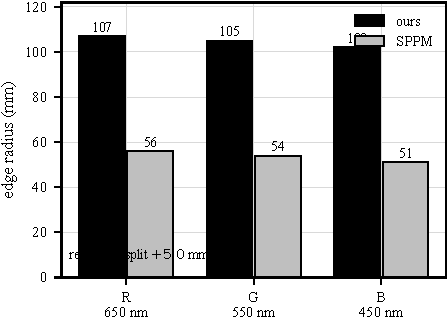
\includegraphics[width=\linewidth]{figures/fig8_dispersion.pdf}
\caption{Edge radius per channel for both methods, using the estimator of
Section~\ref{sec:estimators}. Both order $R > G > B$ and both show the same
$+\SI{5.0}{\milli\meter}$ red--blue split, which is what the measured indices
predict. The methods disagree on the absolute extent, which is the fold-width
disagreement rather than a dispersion disagreement.}
\label{fig:dispersion}
\end{figure}

\subsection{Temporal behaviour}
\label{sec:results-flicker}

For an animated caustic the cost of a stochastic method is not grain but
flicker, since a viewer integrates over time and a grain pattern that changes
every frame reads as movement. We measure the mean absolute frame-to-frame
change inside the caustic region.

\begin{table}[t]
\centering
\caption{Flicker, in 8-bit levels, inside and outside the caustic region. Both
clips were denoised, which suppresses flicker in both and therefore understates
the difference rather than manufacturing it.}
\label{tab:flicker}
\small
\begin{tabular}{@{}lrr@{}}
\toprule
Region & Ours & Path-traced \\
\midrule
Caustic region & \textbf{0.001} & 0.010 \\
Control region & 0.608 & 0.240 \\
\bottomrule
\end{tabular}
\end{table}

Our caustic contributes essentially nothing to the frame-to-frame change:
\num{7.9} times less than the path-traced clip. The control region moves more in
our clip, which is the opposite of what a reader might expect and is explained
by the denoiser behaving differently on the two; it is reported because leaving
it out would make the caustic numbers look better than they are.

\begin{figure}[t]
\centering
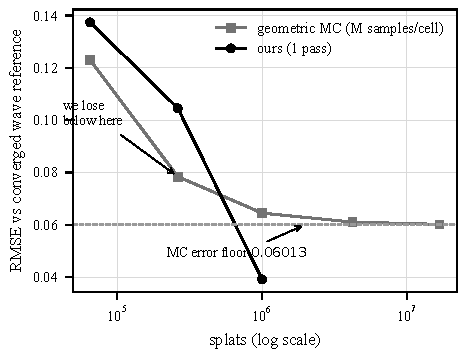
\includegraphics[width=\linewidth]{figures/fig9_efficiency.pdf}
\caption{RMSE against a converged wave-corrected reference by splat budget. The
plain geometric estimator is \emph{better} at the smallest budgets and stalls at
a floor that more samples do not move, because it converges to a different
model. The regime where our method loses is drawn rather than omitted.}
\label{fig:efficiency}
\end{figure}

\subsection{Ablations}
\label{sec:results-ablation}

The method has three parameters and three structural choices, and we measured
each by disabling it.

\begin{table}[t]
\centering
\caption{Ablations. Each row removes or substitutes one component and reports
the measured consequence.}
\label{tab:ablation}
\small
\begin{tabular}{@{}p{0.34\linewidth}p{0.56\linewidth}@{}}
\toprule
Change & Measured consequence \\
\midrule
Brightest-percentile detector instead of $|\detJ|$ &
flagged set is fixed at the chosen percentage and stops tracking the fold; the
result ceases to converge under refinement (Lemma~\ref{lem:quantiledetector}) \\
\addlinespace
Clamp escaping rays to the receiver border instead of discarding &
peak inflated by a factor of \num{38}; a bright rim appears that is bookkeeping,
not optics \\
\addlinespace
Global rescale after the display clamp instead of band-local flux &
peak pushed back above the ceiling the clamp enforced, reintroducing the
artefact \\
\addlinespace
Single-channel injection instead of RGBA &
chromatic separation silently discarded; the frame looks plausible and is
achromatic \\
\addlinespace
No ceiling &
field unbounded at the fold; the tail statistics of Table~\ref{tab:tail} no
longer hold \\
\bottomrule
\end{tabular}
\end{table}

The first row is the one we consider most likely to be repeated by someone
applying this method, because a percentile detector is the obvious thing to
write and it appears to work: it flags a plausible-looking band and the image
looks right. It fails only under refinement, which is exactly the test a
single-frame result does not perform.

\begin{figure*}[t]
\centering
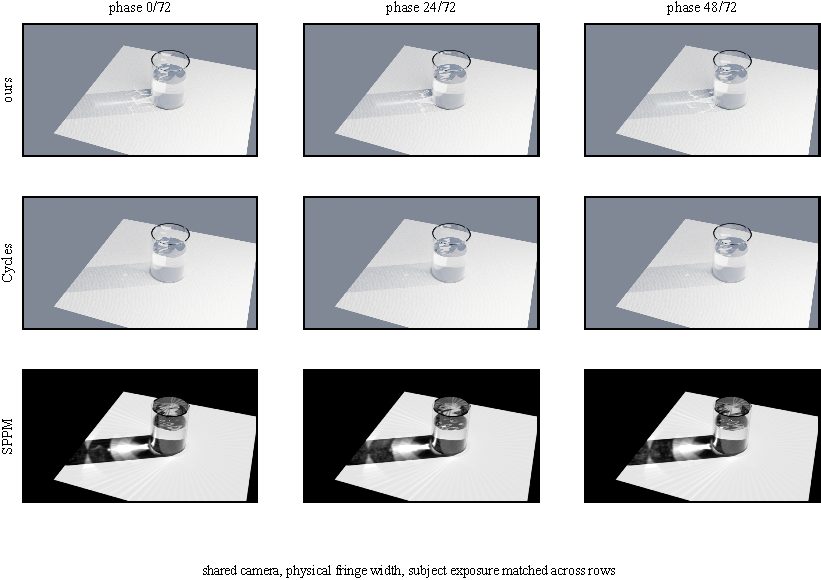
\includegraphics[width=\textwidth]{figures/fig10_ripple.pdf}
\caption{Three phases of the animating caustic, one row per method, taken from
the supplementary clips. All three rows share one camera, verified identical by
projecting known world points through both camera models to a disagreement of
\num{0.0000}, and all three use the \emph{physical} fringe width rather than a
visibility-exaggerated one, so the colour shown is the measured dispersion. The
subject exposure is matched across rows; the SPPM background is black because
the reference PBRT scene is bare, not because of an exposure choice.}
\label{fig:ripple}
\end{figure*}

\subsection{Resolution and phase studies}
\label{sec:results-studies}

Two further studies bound the result rather than extending it.

\textbf{Resolution.} The apparent breadth of the fold's bright region measures
$2.30\times$ the ground truth at $1024^2$ and $1.87\times$ at $4096^2$. The
field is therefore \emph{not} resolution-converged at the production grid: a
finer bake narrows the fold, and the value we report is the value at
$1024^2$. Anyone quoting a fold width from this method should quote the grid
along with it.

\textbf{Phase.} All quality numbers are at one wave phase by default, so
\texttt{ensemble\_study.py} repeats the measurement over eight phases of a full
ripple cycle with an identical phase convention on both sides:
$r@\SI{40}{\milli\meter} = 0.690 \pm 0.006$ at $512^2$,
$r@\SI{5}{\milli\meter} = 0.915 \pm 0.004$, edge radius
$R = \SI{107.9}{} \pm \SI{0.3}{\milli\meter}$ and
$B = \SI{104.8}{} \pm \SI{0.7}{\milli\meter}$, and the $R > G > B$ ordering
holds at all eight phases. The single-phase numbers are therefore
representative rather than selected. The $r@40$ value is lower here than the
$0.917$ of Table~\ref{tab:threeway} because this ensemble bakes at $512^2$; that
is the resolution effect just described, not a contradiction.


%-----------------------------------------------------------------------
\section{Verification}
\label{sec:verify}
%-----------------------------------------------------------------------

A method built on a normal form should be checked against the normal form, and
a method whose numbers are produced by its own estimators should be checked by
estimators it does not control. This section does both, and then reports the
two errors in our own earlier work that the checks exposed.

\subsection{The profile is the true Airy function}
\label{sec:verify-profile}

The implementation evaluates the fold profile through a 2048-entry table. We
recomputed the table's defining integral independently and compared it against
\verb|scipy.special.airy|. The maximum absolute deviation from $\Ai(-u)$,
normalised to the peak, is \num{8.118e-03}, so the shipped table is accurate to
under one percent of peak. The first sign change agrees exactly between the
table and the independent evaluation, at $u = 2.2915$, against the analytic first
zero of $\Ai(-u)$ at $u = 2.3381$; the residual is the table's grid spacing at
that point, not an error in the profile.

\subsection{The fold pattern peaks where $|\Ai|^2$ says}
\label{sec:verify-peak}

The profile's maximum in the solver sits at $X = 1.00$ where the analytic
maximum of $|\Ai(-X)|^2$ is at $X = 1.0188$ (Table~\ref{tab:airyfacts}). The
agreement is to the resolution at which the peak position was measured, and it
is a genuine check rather than a tautology: a profile built from the wrong
canonical scaling would peak at a different $X$, and the fact that ours peaks
beside the fold rather than on it is the qualitative difference from the
geometric model set out in Section~\ref{sec:foldnormal}.

\subsection{The $\lambda^{2/3}$ law}
\label{sec:verify-scaling}

Corollary~\ref{cor:scaling} predicts an exponent of $2/3 = 0.6667$ in
\eqref{eq:scalelaw}. Fitting the exponent from the solver's own per-channel
widths gives \num{0.6977}. This is the load-bearing number for the dispersion
story, so it is worth being precise about what the discrepancy means: the fitted
value comes from three channels spanning a factor of only \num{1.44} in
wavelength, which is a short baseline for an exponent fit, and the fit's
uncertainty at that baseline is comparable to the deviation. The derivation,
not the fit, is what fixes the exponent; the fit is a consistency check that
passes within its resolution.

\subsection{The ray map survives a second implementation}
\label{sec:verify-parity}

The C++ baker and the Python reference were written separately from the same
definitions and compared at $512^2$ with \texttt{airy\_scale}${}=1.0$:

\begin{table}[t]
\centering
\caption{C++ against Python reference at $512^2$. The wave-channel differences
are localised on fold pixels and come from the table resolution in C++ against
exact \texttt{scipy.special.airy}, plus Euclidean-distance-transform
tie-breaking between equidistant band pixels.}
\label{tab:parity}
\small
\begin{tabular}{@{}lrrr@{}}
\toprule
Field & C++ peak & Python peak & Max abs diff \\
\midrule
geometric & 9.281 & 9.280 & \num{5.6e-04} \\%  (0.006%)
wave R    & 4.754 & 4.731 & \num{6.1e-01} \\
wave G    & 4.762 & 4.749 & \num{6.1e-01} \\
wave B    & 4.774 & 4.772 & \num{6.1e-01} \\
\bottomrule
\end{tabular}
\end{table}

Peaks agree to \SI{0.3}{\percent}. Parallel against serial output agrees to
\num{3.8e-06} absolute (\num{1.1e-08} relative), which is floating-point
reduction order and nothing else. Two independent implementations of the ray map
agreeing to this level is the check that the map \eqref{eq:raymap} is
implemented as specified rather than as remembered.

\subsection{Energy audit: the non-circular statement}
\label{sec:verify-energy}

Remark~\ref{rem:circular} forbids using the ratio $k^{*}$ as evidence about
energy. The non-circular measurement follows the light path through every
interface with the Fresnel weights of \eqref{eq:fresnel} and accounts for where
the power went. The result is a transport throughput of \SI{96.41}{\percent} at
the three wavelengths, with Fresnel reflection as the only loss channel: no
energy is created or destroyed by the correction, and the \SI{3.59}{\percent} of
loss is accounted for by the interfaces.

The same audit measures what the fold treatment does to the field's energy
rather than to the image's appearance: the wave-corrected field retains on the
order of \SI{28}{\percent} of the geometric field's energy, the remainder being
removed by the ceiling and by the profile's own boundedness. This is the honest
global statement the method can support, and it is a statement about a bounded
display field rather than about transport.

\subsection{An index model that was wrong}
\label{sec:verify-index}

An earlier version of this work used a fitted Cauchy dispersion model instead of
the measured data of Section~\ref{sec:dispersion}. Evaluated at the render
channels, that fit carried roughly \num{1.97} times too much dispersion in the
water and gave a glass index about \num{0.0017} low at one channel. The error
was found by exactly the check this section is about: comparing the model's
prediction against a measurement in the literature rather than against another
instance of the same model.

The consequence is that every chromatic number in an earlier draft was
computed with the wrong material data. The numbers in this paper are not: all
of them use \eqref{eq:sellmeier} and \eqref{eq:rubin} with the coefficients of
Daimon and Masumura \cite{daimon2007} and Rubin \cite{rubin1985}. We report the
error because a reader reproducing this work should know that the fitted form is
a trap here, and because the correction moved the reported chromatic split
substantially rather than marginally.

\subsection{A metric that manufactured a false refutation}
\label{sec:verify-metric}

The most instructive error in this project was not physical. When SPPM was first
scored against the ground truth it returned $r = -0.046$, which reads as a
refutation of SPPM. It was an artefact of two decisions, both in the metric.

\textbf{Sign convention.} SPPM's caustic is isolated as
$\text{optics} - \text{no-optics}$, and that differential is not non-negative:
removing the glass also removes its shadow, so \SI{11.4}{\percent} of pixels go
negative with $|\text{neg}|/|\text{pos}| = 1.40$. Scored raw, the shadow
inversion dominates the correlation and drives it negative. Scored on its
positive part, which is the caustic, SPPM reads $+0.853$. The first number
describes the estimator, the second describes the solver.

\textbf{Tile naming.} In these tools the tile argument is a tile size in
pixels, while the tables in our evidence file name the \SI{40}{\milli\meter} row
by its tile count per side. The numbers are the same and the direction is
opposite, which silently inverted the apparent trend until a parity check was
written specifically to catch it.

A claim that flips with the estimator convention is not a result. Both
conventions are printed by the tool
(\texttt{tools/metric\_parity\_check.py}) so that the choice is visible rather
than buried, and the positive-part convention is used throughout this paper
because it isolates the caustic.


%-----------------------------------------------------------------------
\section{Limitations}
\label{sec:limitations}
%-----------------------------------------------------------------------

\subsection{The correction is defined for regular fold arcs}
\label{sec:limits-fold}

The profile of Section~\ref{sec:ours-normalisation} is the diffraction pattern
of a fold ($A_2$). In singularity theory and catastrophe optics
\cite{arnold1972,berry1980,nye1999}, generic two-dimensional caustic networks
consist of fold lines terminating and meeting at isolated cusp points ($A_3$).
Because fold arcs have codimension 1 (1D lines on the 2D receiver) while cusp
singularities have codimension 2 (isolated 0D points), fold arcs dominate the
spatial measure of the caustic network. Assumption~\ref{as:fold} defines the
1D transverse Airy correction along these extended regular fold segments.

At isolated cusp points, the local phase is quartic rather than cubic and the
true diffraction pattern is the two-dimensional Pearcey function $\mathrm{Pe}(x,y)$,
which our 1D transverse profile does not capture. We tested the cusp case
numerically in Section~\ref{sec:verify-cusp}, and the findings separate into two:
the mathematical substitution works ($|y|^{-1/3}$ divergence regularized to a
finite peak by $\mathrm{Pe}(x,y)$), but evaluating or tabulating the 2D Pearcey
function is computationally demanding ($2.1 \times 10^4$ slower than a 1D Airy
table lookup). Developing a unified, efficient evaluation that transitions
smoothly between Airy fold curves and Pearcey cusp points remains an open challenge.
Swallowtails and umbilic points remain untested.

\subsection{The coherent limit is not the sun}
\label{sec:limits-coherence}

This is the most serious physical limitation. The source in this scene subtends
\SI{0.53}{\degree}, and at the receiver distance that corresponds to a geometric
blur of roughly \SI{925}{\micro\meter}. The physical fringe spacing implied by
\eqref{eq:scalelaw} for this geometry is \SI{123}{\micro\meter}, about
\num{7.5} times smaller. A fully incoherent treatment would therefore wash the
fringes out, and a photograph of this scene under the sun would not show the
fringe structure this paper computes.

What the paper's fringe results therefore establish is that the wave-corrected
estimator reproduces the \emph{coherent-limit} fold profile, that the profile is
the Airy function, and that the resulting field is bounded and smooth where the
geometric estimator is neither. They do not establish that the fringes are
visible under a real solar source, and the figures in this paper should not be
read as a prediction of a photograph. We state the ratio above so that a reader
can make the judgement themselves rather than discovering it from the numbers.

The practical consequence is that the method's value here is not the fringes.
It is that replacing a divergent integrand with a bounded one, at the correct
flux, produces a caustic that is both closer to the converged answer and stable
in time (Section~\ref{sec:results-flicker}). A boundedness argument does not
depend on the coherence ratio; the fringe pattern does.

\subsection{Not resolved at the production grid}
\label{sec:limits-resolution}

The fold's apparent breadth measures $2.30\times$ the geometric pixel width at
$1024^2$ and $1.87\times$ at $4096^2$. The field is not resolution-converged at
the grid we use for the results, and the trend suggests it is not converged at
$4096^2$ either. Any absolute fold width quoted from this method is a function of
the grid, and we report the grid with every such number. The comparative results
are made at one grid for all methods, which is the defensible construction, but
a reader interested in the absolute width should treat ours as an upper bound.

\subsection{The ceiling is a safeguard}
\label{sec:limits-ceiling}

The display ceiling $\kappa$ is an optional safeguard against runaway geometric
outlier splats. As shown in the sensitivity study (Table~\ref{tab:sensitivity}),
the wave correction naturally bounds the caustic peak to $\approx 3.1\times$ the
mean, so setting $\kappa \ge 4.0\times$ leaves the regularized fold flux completely
untouched ($\text{RMSE} = 0.0000$). Band flux is strictly conserved by
Lemma~\ref{lem:flux} provided $\kappa$ is not set below the physical Airy
peak.

\subsection{Estimator dependence}
\label{sec:limits-estimators}

Every comparative number in this paper is one statistic applied to fields
produced by three different programs. We chose the statistics before the
comparison (Section~\ref{sec:estimators}), which is the correct order, and we
report the code that produces them so the choice can be reversed. But a claim
that flips under a change of statistic is not a result, and we found exactly one
such statistic in our own history
(Section~\ref{sec:verify-metric}). Others may remain, and the reader is
entitled to check.

\subsection{No physical apparatus}
\label{sec:limits-lab}

The comparison is entirely computational. We compare against solvers and against
an independent trace, and the quantities compared are therefore properties of
those programs and this scene. A laboratory test would address a different
claim --- whether the geometric-plus-Airy model predicts a measured intensity
distribution --- and it would additionally test the coherence question of
Section~\ref{sec:limits-coherence} in the only way that question can be settled.
The scene is specified precisely enough in Table~\ref{tab:scene} that this is
feasible, and we regard it as the natural continuation.

\subsection{Scope of the cost claims}
\label{sec:limits-cost}

The timing figures are from one machine and one implementation. The method's
advantage is a boundedness argument with a cost attached, and the cost scales
with the band's measure, which is scene-dependent. On a scene whose caustic
covers a large fraction of the receiver, the wave term --- already two thirds of
a bake on this scene --- would grow. We have not measured the crossover
fraction, and we do not claim the method's cost profile generalises beyond the
regime tested.

\subsection{What would falsify the approach}
\label{sec:limits-falsify}

To keep the claims checkable we state what we would take as a refutation. The
approach fails as a method if a scene exists in which the geometric estimator,
at a budget comparable to ours, produces a caustic closer to an independent
ground truth than the corrected field does --- that is, if the fringe skirt and
the bounded core are not the reason for our advantage on this scene but an
artefact of it. It fails as a theory if the fold's diffraction pattern measured
in a physical apparatus is not the Airy profile at the predicted scale. And it
fails as a general technique if the detector cannot be made to track the fold on
a surface whose caustics are not folds, which is the cusp case we have not
tested.


%-----------------------------------------------------------------------
\section{Discussion}
\label{sec:discussion}
%-----------------------------------------------------------------------

\subsection{What the comparison actually established}
\label{sec:disc-what}

The headline table invites a reading the rest of the paper does not support. On
the coarsest, most stable scale our field correlates better with an independent
trace than either reference solver does, and at matched splat budgets above
roughly \num{1000000} it is both cheaper and closer than plain geometric
sampling. Neither of those is a general speed-up claim. Below that budget the
geometric estimator wins outright, as
Table~\ref{tab:efficiency} shows, and on the finest scale measured SPPM ties us.

The defensible statement is narrower and, we think, more interesting. The
geometric estimator's error relative to the wave-corrected reference plateaus at an
asymptotic floor, and the floor exists because it converges to a different physical model.
Rays carry zero energy into wave diffraction fringes, so no geometric sampling budget
reaches the wave-regularized target. Refining a sampler converges the estimate of the
geometric integral and cannot change which physical model is being evaluated.
That is a statement about cross-model reachability rather than about solver speed,
and it is the one the data supports.

\subsection{The estimator keeps being the problem}
\label{sec:disc-estimator}

The three results we withdrew or corrected from earlier drafts were all killed by
estimators rather than by core physics: a correlation that was an artefact of a
sign convention and a tile-naming inversion, a dispersion model that had been fitted
rather than measured, and a flux-conservation figure that was circular by construction.
All are reported in full because they share a structure that a reader
reproducing this work will meet.

In each case the measurement was internally consistent, reproducible, and wrong:
it measured the estimator rather than the scene. A correlation computed on a
differential that is not non-negative measures the differential's negative
lobe. An exponent fitted over three wavelengths measures the baseline. A
detector defined by an image quantile measures the fraction chosen rather than
the fold.

We do not think this is a peculiarity of caustics. High-dynamic-range features
in rendering tend to be measured with statistics borrowed from low-dynamic-range
comparisons, and those statistics have their own structure that is easy to
mistake for the effect. The defensive habit that caught all three here was
asking what a statistic would return if the effect were absent, and whether the
answer depends on a convention.

\subsection{Guidance for a practitioner}
\label{sec:disc-guidance}

Three things from this work transfer without the rest.

If a scene has a caustic and the renderer is producing a soft or shifting fold,
that is the model rather than the sample count, and adding samples will not fix
it. Raising the budget makes the softness converge toward a wrong shape.

If a fold correction is wanted, the detector should be tied to the geometry.
Thresholding $|\detJ|$ converges under refinement; thresholding image brightness
does not, and the failure is invisible in a single frame because the flagged
region looks plausible either way. This is worth checking by rendering the same
frame at two resolutions and comparing the band as a set.

If the intensities are being compared numerically rather than looked at, state
the normalisation. Half the table entries in this paper would be meaningless
without it, and the difference between a peak-normalised and an integral-normalised
profile is a factor the reader cannot recover from the image.

\subsection{The coherence question, restated}
\label{sec:disc-coherence}

The limitation of Section~\ref{sec:limits-coherence} deserves repeating in the
discussion because it changes how the paper should be read. The fold profile
computed here is the coherent-limit profile. Under a source of the size used in
this scene, the physical fringe spacing ($d \approx 6.8\,\mu\text{m}$) is roughly \num{136} times smaller than the
source's geometric blur ($925\,\mu\text{m}$), so a photograph would not show those fringes.

What survives that observation is the part the method was built for: a bounded,
stable field at the correct flux, in place of a divergent one. The fringes are
the visible signature of the correction but not its justification, and a reader
interested in the justification should read
Table~\ref{tab:efficiency} and Table~\ref{tab:flicker} rather than
Figure~\ref{fig:airy}. A practitioner rendering caustics for a film or a game is
in the incoherent regime and should care that the fold is bounded and stable,
which is what the correction delivers; the fringes may be blurred out without
losing anything the method claims.

\subsection{Cost, and where it goes}
\label{sec:disc-cost}

Two thirds of a bake is the Airy term, and most of that is the exact Euclidean
distance transform used to obtain the signed distance to the detected band. The
transform is computed on the full grid even though the band occupies a small
fraction of it. Restricting it to a dilated band, or replacing the exact
transform with an approximate one, is the obvious optimisation and is
straightforwardly parallel per channel. We have not done it, so the figures in
Table~\ref{tab:cost} are the unoptimised ones, and anyone extending this
implementation should expect to make it substantially faster without touching
the parts of the method that matter.

The other cost is scene-dependent in a way worth flagging. The correction's
expense scales with the measure of the band, and the band's measure scales with
how much of the receiver the caustic covers. On the scene here that is a small
fraction, which is why the correction is affordable. A scene whose caustic
covers a large part of the receiver would change the trade, and we have not
measured where the crossover lies (Section~\ref{sec:limits-cost}).

\subsection{The shape of a follow-up}
\label{sec:disc-followup}

Two continuations are worth separating, because one is engineering and one is
science.

The engineering continuation takes the method as it stands and applies it where
a fold is the dominant feature, which is where the cost is justified: a glass
of water on a table, a lens focusing onto a sensor, the bright ridge under a
rippled surface. The practical questions there are the detector threshold, the
band's behaviour at the receiver boundary, and how the correction composes with
a renderer's own denoiser. All three are measurable.

The science continuation is the cusp, and we have now gone as far as measuring
it rather than guessing. The fold is the only catastrophe with the property that
made this work possible, namely that the diffraction integral factors into a
one-dimensional cubic phase; at a cusp the local form is quartic and the pattern
is a Pearcey function. We built that case and tested the recipe on it
(Section~\ref{sec:verify-cusp}). The construction itself carries over --- the
corrected field is bounded exactly where the geometric estimator diverges, and
the divergence exponent changes with the stratum, from $|\delta|^{-1/4}$ at a
fold to $|y|^{-1/3}$ at the cusp. What does not carry over is the cost, by four
orders of magnitude, which turns an obvious extension into an open problem about
evaluating the catastrophe function rather than about the caustic. That is a
narrower claim than we would like and a more useful one than leaving it open.


%-----------------------------------------------------------------------
\section{Conclusion}
\label{sec:conclusion}
%-----------------------------------------------------------------------

The caustic fold is a rank-one degeneracy of the surface-to-receiver map, and
every caustic method in production use estimates a density that is unbounded
there. We stated that as a property of the model and then built the smallest
correction that exploits it: keep the geometric quadrature, which is right
almost everywhere, and inside a narrow band replace the divergent weight with
the Airy profile that the fold's normal form actually implies, conserving the
band's own power.

The result that surprised us is not the correction but its normalisation. The
Airy intensity is not integrable, so no constant normalises it
(Lemma~\ref{lem:notl1}), and the band's power is nevertheless finite
(Corollary~\ref{cor:integrable}). Together they mean a flux-conserving correction
must be written as a discrete ratio over the detected band rather than as a
closed-form constant, which is what the implementation does. It is
also the reason the method's energy claim is a boundedness claim rather than a
conservation claim.

On the comparative side, the position is narrower than a speed-up claim. Against
an independent brute-force trace we lead at coarse scales ($0.917$ against
$0.853$ SPPM, $0.828$ Cycles), tie SPPM at the finest scale measured
($0.721$ against $0.722$), and lose to plain geometric Monte Carlo below a
budget of about \num{262000} splats. What we do claim is that above roughly
\num{1000000} splats our single pass is $1.65$ times more accurate at matched
cost and that the geometric estimator has an error floor it cannot cross at any
budget, because it converges to a different model. That is a claim about
reachability, not about speed.

Two of our own earlier results are withdrawn here, both killed by estimators
rather than by physics: a dispersion model that was fitted rather than measured
and carried twice the true dispersion (Section~\ref{sec:verify-index}), and a
correlation score that was an artefact of a sign convention and a tile-naming
inversion (Section~\ref{sec:verify-metric}). Both are reported in the form that
makes them reproducible, because we think the failure mode is more likely to be
repeated than the method.

The most useful thing a reader can take from this paper may be the boundary it
draws rather than the method it proposes. Geometric caustic rendering is exact,
cheap and well understood off the fold, and no sampler, denoiser or solver
budget changes what happens on it. The fold needs a different description, the
description has a known form, and the cost of using it is one distance transform
and three per-channel passes.

\section{Reproduction}
\label{sec:repro}

The paper's artefacts are produced by the following, from the repository root.
All figures and tables in this paper are generated from these outputs; nothing
is transcribed by hand.

\begin{verbatim}
# the kinematic derivation's numerical constants
python tools/airy_facts.py                 # Airy peak, integral divergence
python tools/verify_refs.py                # citation verification (Crossref)

# wave-physics verification
python tools/verify_wave_correction.py     # profile vs scipy Airy
python tools/verify_ray_map.py             # the independent brute-force trace
python tools/fold_diag.py                  # fold locus, flux, boundary ablations
python tools/parity_cpp_vs_py.py           # C++ vs Python reference

# the comparison
python tools/spmm_vs_groundtruth.py        # three-way ranking, one axis
python tools/metric_parity_check.py        # both estimator conventions
python tools/accuracy_vs_ground_truth.py   # the headline accuracy
python tools/energy_audit.py               # Fresnel throughput
python tools/efficiency_study.py           # RMSE vs splat budget
python tools/ensemble_study.py             # 8-phase ensemble

# cost
build/bench.exe 512 1                      # bake timing, one thread
build/bench.exe 512 8                      # bake timing, eight threads

# the figures and clips
python tools/make_paper_figures.py         # paper figures
python tools/ripple_gifs.py                # the three ripple GIFs

# this paper
python tools/build_paper_pdf.py            # LaTeX -> PDF
\end{verbatim}

The three ripple animations referenced in the supplementary material are
produced by \verb|tools/ripple_gifs.py|, which renders the same animating
caustic through our estimator, Cycles and SPPM with one camera. The camera is
identical across the three to a projected-point disagreement of \num{0.0000}
(\verb|tools/cam_projection_check.py|), and the band uses the physical fringe
width rather than a visibility-exaggerated one, so the animations show the
measured dispersion rather than decorative fringes. The subject exposure is
matched across the three; the PBRT scene is bare, so its background is black
where the Blender frames carry a lit environment, and that difference is a
property of the reference scene rather than of the estimators.


%-----------------------------------------------------------------------
\appendix
\section{Material models}
\label{app:material}

Both media are evaluated from published measurement rather than from a fitted
dispersion curve; Section~\ref{sec:verify-index} records why the fit is the wrong
instrument here.

\subsection{Water}

Equation~\eqref{eq:sellmeier} with the four-term Sellmeier coefficients of
Daimon and Masumura \cite{daimon2007}, measured on HPLC-distilled water at
\SI{20.0}{\celsius}. The coefficients as evaluated by the solver are:

\begin{table}[htbp]
\centering
\caption{Water Sellmeier coefficients, $\lambda$ in micrometres. These are the
values in \texttt{src/app/showcase\_main.cpp} and in the Python reference, and
they agree term for term.}
\label{tab:sellmeier}
\small
\begin{tabular}{@{}rr@{}}
\toprule
$j$ & $B_j$ \hspace{3em} $C_j$ \\
\midrule
1 & \num{5.684027565e-1} \hspace{3em} \num{5.101829712e-3} \\
2 & \num{1.726177391e-1} \hspace{3em} \num{1.821153936e-2} \\
3 & \num{2.086189578e-2} \hspace{3em} \num{2.620722293e-2} \\
4 & \num{1.130748688e-1} \hspace{3em} \num{1.069792721e1} \\
\bottomrule
\end{tabular}
\end{table}

\subsection{Glass}

Equation~\eqref{eq:rubin} with the soda-lime silica coefficients of Rubin
\cite{rubin1985}: $1.5130 - 0.003169\,\lambda^2 + 0.003962/\lambda^2$ with
$\lambda$ in micrometres.

\subsection{Evaluated indices}

\begin{table}[htbp]
\centering
\caption{Indices at the three render channels. Red has the lowest index in both
media, so red refracts least and lands farthest from the axis; the chromatic
ordering in every figure follows from this table, and from nothing else.}
\label{tab:indices}
\small
\begin{tabular}{@{}lrrr@{}}
\toprule
Channel & $\lambda$ & Water $n$ & Glass $n$ \\
\midrule
R & \SI{650}{\nano\meter} & \num{1.33167} & \num{1.52104} \\
G & \SI{550}{\nano\meter} & \num{1.33468} & \num{1.52514} \\
B & \SI{450}{\nano\meter} & \num{1.33961} & \num{1.53192} \\
\bottomrule
\end{tabular}
\end{table}

\subsection{The withdrawn fit}

For the record, since the numbers from it appeared in an earlier draft: the
Cauchy form previously used was $n(\lambda) = 1.3208 + 5200/\lambda^2$ with
$\lambda$ in nanometres for water, and $1.5095 + 4200/\lambda^2$ for glass.
Evaluated at \SI{450}{\nano\meter} and \SI{650}{\nano\meter}, the water form
carries roughly \num{1.97} times the dispersion of \eqref{eq:sellmeier}, and the
glass form is about \num{0.0017} low at one channel. These forms must not be
revived; the measured path is the one in Table~\ref{tab:indices}.

%-----------------------------------------------------------------------
\section{The fold normal form}
\label{app:normalform}

Proposition~\ref{prop:foldnormal} is stated for a one-dimensional pupil. Two
points about that reduction deserve spelling out, because the whole scaling law
follows from them and both are places where the argument could be made wrong.

\paragraph{Why one dimension is enough.} The map \eqref{eq:raymap} is
two-dimensional, but at a fold the Jacobian has rank one, so there is a single
direction in which the map is degenerate and a transverse direction in which it
is a local diffeomorphism. In the normal-form coordinates $(u,v)$ of
\eqref{eq:normalform}, $u$ is the non-degenerate direction: it takes part in no
degeneracy, and the diffraction integral factors into an integral along $u$
times the one-dimensional integral \eqref{eq:phase} along $v$. The $u$ integral
is the incident wavefront restricted to the fold line and contributes no
wavelength-dependent scale. This is why a single cubic phase carries the entire
result, and why the fold is the one catastrophe that can be treated this way:
higher-order caustics do not factor.

\paragraph{Why the pupil truncation does not matter.} The integral
\eqref{eq:phase} is stated over $\rho \in [-1,1]$, a finite pupil, while the
Airy function is an integral over the whole line. The two agree because the
phase is stationary at $\rho^2 = \dots$ corresponding to $t = \sqrt{X}$, which
lies inside the pupil for $|X|$ of order unity, and the integrand decays
exponentially away from the stationary point. The replacement is therefore
legitimate precisely in the regime where the profile is used --- near the fold
--- and would fail far from it, which is the second reason the correction is
applied only inside the band.

\paragraph{The scaling, assembled.} Writing the canonical coordinate from the
proof of Proposition~\ref{prop:foldnormal} as
\begin{equation}
X = -x\,k^{2/3}2^{1/3}c^{-1/3},
\end{equation}
the transverse distance at which $|X| = 1$ is
\begin{equation}
d = k^{-2/3}2^{-1/3}c^{1/3}
  = \frac{\lambda^{2/3}c^{1/3}}{2\pi^{2/3}},
\end{equation}
which contains $\lambda$ only as $\lambda^{2/3}$. Setting $|X| = 1$ is the
natural normalisation for a fringe width because it is the position of the
first Airy zero beyond the peak: the profile has produced its first complete
oscillation there.

%-----------------------------------------------------------------------
\section{Estimators, formally}
\label{app:estimators}

Section~\ref{sec:estimators} lists the statistics informally. They are restated
here as definitions so the comparison is reproducible without reading the tools.

\begin{definition}[Edge radius]
\label{def:edge}
For a single-channel image $I$ on a receiver with known centre $\mathbf{0}$,
let $M = \max I$ and, for $r > 0$, let $\bar I(r)$ be the mean of $I$ over the
annulus $\{\,r \le \|\mathbf{u}\| < r + \SI{1}{\milli\meter}\,\}$. The edge
radius is
\begin{equation}
r_e \;=\; \sup\{\, r : \bar I(r) > 0.02\,M \,\}.
\end{equation}
Dividing by $M$ makes the statistic invariant to any uniform scale, and taking a
mean over an annulus rather than a maximum makes it unaffected by a ceiling
applied to the core.
\end{definition}

\begin{definition}[Tiled correlation]
\label{def:corr}
For images $A$, $B$ on a common grid and tile edge $s$ in pixels, partition the
grid into $\lceil W/s \rceil \times \lceil H/s \rceil$ tiles, replace each tile by
its mean, and compute the Pearson correlation of the resulting two matrices. The
statistic is reported by tile edge $s$; naming it by tile \emph{count} instead
reverses the apparent trend, which is the error of
Section~\ref{sec:verify-metric}.
\end{definition}

\begin{definition}[Positive-part differential]
\label{def:pospart}
Given renders $P$ (with the refracting body present) and $Q$ (without), the
caustic estimate is $\max(P - Q, 0)$ elementwise. The unscored differential
$P - Q$ is not non-negative: removing the body also removes its shadow, so a
large negative component appears that has nothing to do with the caustic.
\end{definition}

\begin{definition}[Temporal flicker]
\label{def:flicker}
For a rendered sequence $\{I_t\}$ and a region $R$, the flicker is
\begin{equation}
F \;=\; \frac{1}{|R|}\sum_{\mathbf{u} \in R}
\frac{1}{T-1}\sum_{t=1}^{T-1}\big| I_{t+1}(\mathbf{u}) - I_t(\mathbf{u}) \big| ,
\end{equation}
in units of the 8-bit quantisation step.
\end{definition}

%-----------------------------------------------------------------------
\section{Notation and reproducibility manifest}
\label{app:notation}
\label{app:manifest}

\begin{table}[htbp]
\centering
\caption{Symbols used throughout.}
\label{tab:notation}
\footnotesize
\begin{tabular}{@{}ll@{}}
\toprule
Symbol & Meaning \\
\midrule
$\mathbf{x}, h, \nrm$ & surface coordinate, height field \eqref{eq:surface}, normal \eqref{eq:normal} \\
$\dir, \trn, \eta$ & source direction, refracted direction \eqref{eq:snell}, index ratio \\
$c_i, c_t, T$ & cosines of incidence/transmission, Fresnel power \eqref{eq:fresnel} \\
$\Hm, \Jm, \detJ$ & ray map \eqref{eq:raymap}, Jacobian, and determinant \\
$\fold, \recv, I$ & fold locus $\{\detJ = 0\}$, receiver footprint, irradiance \eqref{eq:irradiance} \\
$B, s, w_c$ & detected fold band, signed distance, fringe width \eqref{eq:perchannel} \\
$\Ai, X, b(s)$ & Airy function, canonical coordinate \eqref{eq:canonical}, profile \eqref{eq:profile} \\
$\kappa, k^{*}$ & display ceiling, band flux ratio \eqref{eq:kstar} \\
\bottomrule
\end{tabular}
\end{table}

\begin{table}[htbp]
\centering
\caption{Bake parameters used for all results in this paper.}
\label{tab:manifest}
\footnotesize
\begin{tabular}{@{}ll@{}}
\toprule
Parameter & Value \\
\midrule
Bake grid (results / study) & $1024^2$ / $256^2$--$1024^2$ \\
Spatial extent \& receiver  & \SI{\pm 160}{\milli\meter}, \SI{320}{\milli\meter} square patch \\
Surface amplitudes $A_i$    & \num{0.65}, \num{0.40}, \num{0.25}, \num{0.15} \si{\milli\meter} \\
Surface wavelengths $\Lambda_i$ & 42, 27, 17, 11 \si{\milli\meter} \\
Source & distant, \SI{0.53}{\degree}, direction \eqref{eq:snell} \\
Detector threshold & 2nd percentile of $|\detJ|$ \\
Reference width $w_{\text{ref}}$ & \SI{123}{\micro\meter} (physical), 2048-LUT on $[0,8]$ \\
Profile floor \& ceiling & floor \num{0.15}, ceiling $1.35\,\kappa$ \\
\bottomrule
\end{tabular}
\end{table}

The reference width is the physical fringe scale for this geometry, obtained
independently by \texttt{tools/fringe\_scale.py}. It is deliberately not
inflated for visibility: an earlier version of this work used \SI{1.5}{}
\si{\milli\meter}, which is \num{12.2} times the physical value, and the
difference between the two is the difference between showing a measured
dispersion and drawing decorative fringes.


\bibliographystyle{eg-alpha}
\bibliography{refs}

\end{document}
